% !TEX program = xelatex

\documentclass{article}
\usepackage[utf8]{inputenc}
\usepackage[T1]{fontenc}
\usepackage{lmodern}
\usepackage[czech]{babel}
\usepackage[top = 2cm, bottom = 2cm, left = 2cm, right = 2cm]{geometry}
\usepackage{calc} % pro \mask

\renewcommand{\baselinestretch}{1.2} % výška řádku

\setcounter{secnumdepth}{2} % aby se \subsubsection nečíslovalo

\usepackage{amsmath}
\numberwithin{equation}{section} % číslování rovnic
\usepackage{amssymb}
\usepackage{mathtools}
\usepackage{amsthm}
\usepackage{xcolor} % barvičky v rovnicích
\usepackage{mathrsfs} % pro spojité operátory \mathsrc{L}
\usepackage[shortlabels]{enumitem} % enumerate a),b)..., pokračování v seznamu [resume]
\usepackage{MnSymbol,wasysym} % smajlíci jsou důležití
\usepackage{diagbox} %škrtání políček v tabulce \diagbox{$a_i$}{$b_j$}
\usepackage[hidelinks]{hyperref} %Dobrá praxe tento balíček nahrát jako poslední.
\usepackage{tikz}
\usepackage{enumitem}
\newcommand{\e}[1]{\const{e}^{#1}}
\newcommand{\I}{\const{i}}

\newcommand{\N}{\mathbb{N}}
\newcommand{\Z}{\mathbb{Z}}
\newcommand{\Q}{\mathbb{Q}}
\newcommand{\R}{\mathbb{R}}
\newcommand{\C}{\mathbb{C}}
\newcommand{\K}{\mathbb{K}}
\newcommand{\Sp}{\reflectbox{S}}

\newcommand{\uu}[1]{\underline{#1}}

\def\ph{\phantom}
\def\vph{\vphantom}
\def\hph{\hphantom}
\def\rzw{\mathrlap}
\def\lzw{\mathllap}
\def\czw{\mathclap}

\newcommand*{\mask}[2]{%
    \mathord{\makebox[\widthof{\(#1\)}]{\(#2\)}}%
}

\title{Vybrané partie z funkcionální analýzy}
\author{Mirko Rokyta (do {\TeX}u přepsal kol.)}
\date{Srpen 2020}


%Věty
\newtheorem{theorem}{Věta}[section]
\theoremstyle{definition}
\newtheorem{definition}[theorem]{Definice}
\newtheorem{lemma}[theorem]{Lemma}
\newtheorem*{remark}{Poznámka}
\newtheorem*{example}{Příklad}
\newtheorem{corollary}[theorem]{Důsledek}
\newtheorem*{exercise}{Cvičení}

\newcommand{\lboxed}[1]{\begin{tabular}{|l}#1\end{tabular}}

\newcommand{\Priklad}[1]{
    \noindent
    \lboxed{
    \fbox{\textbf{Příklad}} \;
    \parbox[t]{\textwidth - 7em}{#1}
    }
}


\newcommand{\Cviceni}[1]{
    \noindent
    \fbox{\textbf{Cvičení}} \;
    \parbox[t]{\textwidth - 7em}{#1}
}
\newcommand{\Poznamka}{
\noindent\uu{Pozn.}: }


% Konstanty
\newcommand{\const}[1]{\mathrm{#1}}
% Norma
\newcommand{\norm}[1]{\left\lVert#1\right\rVert}
% Komplexní sdružení
\newcommand{\conj}[1]{\overline{#1}}
% Skalární součin a symetrie
\newcommand{\innerprod}[2]{\big( #1, #2 \big)}
\newcommand{\duality}[2]{\big< #1, #2 \big>}
% Spojité operátory
\newcommand{\lin}{\mathscr{L}}
% Kompaktní operátory
\newcommand{\comp}{\mathscr{C}}
% Zobrazení
\newcommand{\map}[1]{\boldsymbol{#1}}
% Posloupnost
\newcommand{\sequence}[2]{ \left \lbrace #1 \right \rbrace_{#2=1}^\infty}

% Názvy používaných operací
\newcommand{\arctg}{\operatorname{arctg}\,}
\newcommand{\sgn}{\operatorname{sgn}\,}
\newcommand{\Lin}{\operatorname{Lin}\,}
\newcommand{\Id}{\operatorname{Id}\,}
\newcommand{\Ker}{\mathrm{ker}\,}

% Diferenciál a derivování
\renewcommand{\d}[1]{\;\const{d}#1}
\newcommand{\dd}[2]{\frac{\const{d} #1}{\const{d} #2} \;}
\newcommand{\pd}[2]{\frac{\partial  #1}{\partial  #2} \;}

%random pomůcky
\newcommand*\circled[1]{\tikz[baseline=(char.base)]{
            \node[shape=circle,draw,inner sep=2pt] (char) {#1};}}


\begin{document}

\maketitle


\begin{table}[h!]
\begin{tabular}{l|l}
$\conj{z}$
& číslo komplexně sdružené k $z$
\\
$\mathcal{C}(\Omega), \; \mathcal{C}^k(\Omega)$
& prostor spojitých funkcí ($k$-krát spojitě diferencovatelných funkcí) na množině $\Omega$
\\
$L^p(\Omega), \; L^p_\rho(\Omega)$
& (vážený) Lebesgueův prostor na množině $\Omega$ (s váhou $\rho$)
\\
$W^{k,p}(\Omega), \; W^{k,p}_\rho(\Omega)$
& (vážené) Sobolevovy prostory na množině $\Omega$ (s váhou $\rho$)
\\
$\lin(X, Y), \; \lin(X)$
& prostor spojitých lineárních operátorů mezi prostory $X, Y$ (na prostoru $X$)
\\
$\comp(X, Y), \; \comp(X)$
& prostor kompaktních lineárních operátorů mezi prostory $X, Y$ (na prostoru $X$)
\\
$\mathcal{U}(x)$
& blízké okolí bodu $x$
\\
$\mathcal{D}(\map T)$
& definiční obor operátoru $\map T$
\\
$\mathcal{R}(\map T)$
& obor hodnot (range) operátoru $\map T$
\\
$\mathcal{M}^{n\times m}$
& množina všech $m\times n$ rozměrných matic nad $\R(\C)$
\\
$\map T: X \to Y$
& operátor z $X$ do $Y$
\\
$\Sp(\map T)$
& spektrum operátoru $\map T$
\\
$\innerprod{f}{g}, \; \duality{f}{\map T}$
& skalární součin, dualita
\end{tabular}
\end{table}
\section{Operátorová trivia}

Co budeme považovat za známé:
\begin{itemize}
    \item \emph{Vektorový prostor} $X$ nad
    %\footnote{Zde $X$ je množina a~$\K$ je těleso.}
    % imo je tenhle footnote divně formulovaný a nadbytečný -Michal
    $\underbrace{\R\text{ nebo }\C}_{\text{skaláry}}$ (ale existují i skaláry z $\mathbb{Q}$). Tam, kde nebude důležité, jestli jde o~$\R$ nebo o~$\C$, budeme někdy používat značení $\K$ (znamenající tedy „buď $\R$ nebo $\C$“). Kromě termínu „vektorový prostor“ (VP) se používá i termín „lineární prostor“ (LP), případně „lineární vektorový prostor“ (LVP).
    
    \item \emph{Lineárně nezávislá} (LN) \emph{množina} ve VP: $M \subseteq X$ je LN, pokud $a_1 x_1 + \dots + a_n x_n = 0 \implies a_1 = a_2 = \dots = a_n = 0$ pro všechny možné n-tice $(x_1, \dots x_n) \subseteq M$ a všechny skaláry $a_j \in \K$.
    \\[5pt]
    \Poznamka I v případě, že $M$ je nekonečná, uvažujeme pouze konečné součty (tj. všechny možné „libovolně dlouhé, ale konečné“ součty). Je totiž potřeba si uvědomit, že v~obecném VP není definován pojem konvergence, a~tedy samotný pojem nekonečného součtu nemá v~obecném VP smysl.
    \\[5pt]
    „Konečné součty patří do algebry, nekonečné do analýzy.“
    
    \item \emph{Báze $X$} ($X \neq \emptyset$, $X \neq \{0\}$):
    \begin{enumerate}
        \item Pokud existuje \emph{konečná} LN množina $B$ v~$X$ taková, že její lineární obal
        $$ \Lin(B) \coloneqq \big\{ \sum_{j=1}^n a_j x_j, \;  x_j \in B, a_j \in \K, n \in \N \big\} $$
        je roven $X$ (říkáme, že $B$ \emph{generuje} $X$), pak takovou množinu nazvu \emph{bází $X$}.
        Její mohutnost je pak určena jednoznačně (lze ukázat), tomuto číslu pak říkáme \emph{dimenze $X$}: $\dim X \coloneqq \operatorname{moh}(B) \in \N$.
        \item Pokud $\forall n \in \N$ v $X$ existuje LN množina o $n$ prvcích, říkáme, že $\dim X = \infty$. V tomto případě je pojem báze striktnější: bází $X$ nad $\K$ je v tomto případě taková nekonečná množina $B$, která splňuje:
        \begin{enumerate}
            \item $B$ je LN (ve smyslu všech konečných lin. kombinací – viz výše).
            \item $\forall x \in X \; \exists n(x) \in \N$ a odpovídající konečný počet prvků báze $x_1, \dots,  x_{n(x)}$ a koeficientů $a_j \in \K$, že
            $$ x = \sum_{j=1}^{n(x)} a_j x_j \,. $$
        \end{enumerate}
        
        \Poznamka I zde tedy jde principiálně o konečné součty prvků, vybíraných z nekonečné množiny (pro různá $x$ může jít o různé sady prvků báze). Této nekonečné bázi se říká \emph{Hammelova báze $X$ nad $\K$}. Otázka zní, zda každý VP $X$ (který není konečné dimenze) má Hammelovu bázi. Odpověď \textit{ano} je důsledkem \emph{axiomu výběru} (kdo jej tedy neuznává, pro něj by odpověď byla \textit{ne}).
    \end{enumerate}
\end{itemize}

\Priklad{
    $\underbrace{\R}_{\text{VP}}$ nad $\underbrace{\R}_{\text{skaláry}}$ má dimenzi 1: $\forall x \in \R \exists a = x \in \R$, že $x = a \cdot 1$. Báze je tedy $\{ 1 \}$.
    \\ \\
    $\underbrace{\R^n}_{\text{VP}}$ nad $\underbrace{\R}_{\text{skaláry}}$ má dimenzi $n$.
    \\ \\
    $\underbrace{\R}_{\text{VP}}$ nad $\underbrace{\Q}_{\text{skaláry}}$ má dimenzi $\infty$: totiž každá konečná báze reálných čísel generuje pomocí spočetné množiny koeficientů ($\Q$) jen spočetně mnoho prvků, a $\R$ je nespočetná.

    
    Tím je vyřešen problém dimenze $\R$ nad $\Q$. Všimněte si, že dimenzi $\infty$ lze určit i bez znalosti odpovědi na otázku existence báze, tj. bez nutnosti axiomu výběru. Pokud však připustíme axiom výběru, pak existuje Hammelova báze $\R$ nad $\Q$, tj. $\exists B \subset \R$, že $B$ je LN ve smyslu výše uvedené definice a~$
    \forall x \in \R \;
    \exists n(x) \in \N \;
    \exists b_1, \dots, b_{n(x)} \in B \;
    \exists q_1, \dots, q_{n(x)} \in \Q
    $,
    že $x = \sum_{j=1}^{n(x)} q_j b_j$.
    Rozmyslete si, že B je nutně nespočetná (jinak vygeneruji jen spočetně mnoho prvků).
    }


\begin{itemize}
    \item \emph{Norma na LP}: \hspace{1em}
    $\norm{\cdot}: X \to \R$, že \parbox[t]{20em}{
        $\norm{x+y} \leq \norm{x} + \norm{y}$, \\[3pt]
        $\norm{ax} = |a| \cdot \norm{x}$, \\[3pt]
        $\norm{x} = 0 \iff x = 0$.
    }
    
    $(X, \norm{\cdot})$ je potom normovaný lineární prostor (NLP). V něm lze definovat konvergenci:
    $$
        x_n \xrightarrow{\norm{\cdot}} x
        \iff
        \forall \varepsilon \! > \! 0 \;\;
        \exists n_0 \!\in\! \N \;\;
        \forall n \!\geq\! n_0 \;\;
        \norm{x - x_n} < \varepsilon
    $$
    a lze tedy zavést i nekonečné součty.
    Dále lze definovat cauchyovskost
    $$
        \{ x_n \} \text{ cauchyovská }
        \iff
        \forall \varepsilon \! > \! 0 \;\;
        \exists n_0 \!\in\! \N \;\;
        \forall m,n \!\geq\! n_0 \;\;
        \norm{x_m - x_n} < \varepsilon
    $$
    a \emph{úplnost $X$ v normě}:
    $$
        (X, \norm{\cdot}) \text{ je úplný v normě } \norm{\cdot}
        \iff
        \left(
        \{ x_n \} \text{ cauchyovská }
        \implies
        \exists x \in X \; x_n \to x
        \right)\,.
    $$
    Je-li $(X, \norm{\cdot})$ úplný v normě $\norm{\cdot}$, nazývá se \emph{Banachův} prostor (B-prostor).
    
    \item Za známé dále považujeme, že pokud $\dim X < \infty$, pak všechny normy na něm jsou ekvivalentní. Normy $\norm{\cdot}_1$ a $\norm{\cdot}_2$ nazveme ekvivalentní, pokud $\exists c_1, c_2 > 0$, že
    $c_1 \norm{x}_1 \leq \norm{x}_2 \leq c_2 \norm{x}_1 \; \forall x \in X$.
    
    \item Ekvivalentní normy zachovávají pojem konvergence ($x_n \xrightarrow{\norm{\cdot}_1} x \iff x_n \xrightarrow{\norm{\cdot}_2} x$) i~cauchyovskosti, a~tedy i~úplnosti. Speciálně, je-li konečnědimenzionální prostor $X$ úplný v $\norm{\cdot}$, je úplný i~ve všech jiných možných normách na $X$.
    
    To neplatí v nekonečné dimenzi, např $\mathcal{C}([-1, 1])$ je úplný v maximové normě $\norm{f}_\infty \coloneqq \max_{[-1, 1]} |f(x)|$, ale není úplný v integrální normě $\norm{f}_1 \coloneqq \int_{-1}^1 |f|$. $\big(\arctg nx \to \frac{\pi}{2} \sgn x$ v $\norm{\cdot}_1\big)$
    
    \item \emph{Skalární součin na LP}: $\; \innerprod{\cdot}{\cdot}: X \times X \to \K \;$ (je-li $X$ nad $\C$, má tedy skalární součin komplexní hodnoty), je takové zobrazení, že $\forall x, y, z \in X$ platí:
    \begin{gather*}
        \innerprod{x}{y} = \conj{\innerprod{y}{x}},
        \\[3pt]
        \innerprod{x+y}{z} = \innerprod{x}{z} + \innerprod{y}{z},
        \\[3pt]
        \innerprod{x}{x} \geq 0,
        \text{ přičemž }
        \innerprod{x}{x} = 0
        \iff x = 0,
        \\[3pt]
        \innerprod{\alpha x}{y} =
        \alpha \, \innerprod{x}{y}
        \;\; \forall \alpha \in \K.
    \end{gather*}
    
    \item Prostor $\big(X, \innerprod{\cdot}{\cdot}\big)$ obdařený skalárním součinem se zve LP skalárním součinem, někdy též \emph{unitární prostor}.
    
    \item Snadno lze ukázat, že výraz $\norm{x} = \sqrt{\innerprod{x}{x}}$ má všechny vlastnosti normy, a tedy:
    
    $X$ je unitární $\implies$ $X$ je NLP (v~tzv. \uv{normě generované skalárním součinem})
    
    \item Pokud je $X$ \emph{úplný v normě generované skalárním součinem}, říká se mu \emph{Hilbertův prostor} (H-prostor), tedy:
    
    $X$ Hilbertův $\implies$ $X$ Banachův
    
    \item Na libovolném unitárním prostoru platí \emph{Cauchy-Schwarzova nerovnost}:
    $$
        \forall x,y \in X:
        \hspace{2em}
        |\innerprod{x}{y}| \leq \norm{x} \cdot \norm{y},
        \hspace{2em}
        \text{kde }
        \norm{x} = \sqrt{\innerprod{x}{x}}.
    $$
    
    \item $X$ unitární, řekneme, že $x,y \in X \textbackslash \{0\}$ jsou \emph{kolmé} v $X$ (v odpovídajícím sk. součinu), pokud $\innerprod{x}{y} = 0$. Značíme $x \perp y$.
\end{itemize}

\Priklad{
    $L^2,\, L^2_\rho,\, \ell_2,\, W^{1,2},\, W^{k,2},\, W^{k,2}_\rho$ jsou Hilbertovy.
    \\
    $\mathcal{C}(\K),\, L^p$ pro $p \neq 2$ jsou Banachovy a nejsou Hilbertovy.
    \\ \\
    Existence normy (sk. součinu, příp. metriky) definuje na LP tzv. geometrické vlastnosti (vzdálenost, konvergence, pro sk. součin i kolmost).
}

\phantom{.}

Nyní připomeneme různé pojmy a vlastnosti související se zobrazeními na vektorových prostorech.
\begin{enumerate}
    \item Buďte $X,Y$ LP (tj. nepotřebuji geometrii).
    \begin{itemize}
        \item \emph{operátor}: $\map T: X \to Y$
        \item \emph{funkcionál}: $\map T: X \to \K$
    \end{itemize}
    Každý funkcionál je i operátor. Budeme tedy BÚNO definovat další vlastnosti pro operátory.
    
    \item Operátor $\map T: X \to Y$ je
    \begin{itemize}
        \item \emph{lineární}: $\map T(ax + by) = a \map T(x) + b \map T(y) \hspace{2em} \forall x,y \in X \; \forall a,b \in \K$
        \item \emph{nelineární}: není lineární
    \end{itemize}
    
    \Poznamka z linearity $\map T$ plyne, že $\map T(0) = 0$ (volte $a=b=0$).
    
    \item $X$, $Y$ NLP, $\map T: X \to Y$ je
    \begin{itemize}
        \item \emph{omezený}: $\forall K\!>\!0 \;\; \exists C\!>\!0 \;\; \norm{x}_X \leq K \implies \norm{\map Tx}_Y \leq C$ (zobrazuje se „omezená množina na omezené“),
        
        ekvivalentně $\exists C\!>\!0 \;\; \forall x \!\in\! X \;\; \norm{\map Tx}_Y \leq C \norm{x}_X $.
        
        \item \emph{neomezený}: není omezený, tj. $\exists K\!>\!0 \;\; \forall C\!>\!0 \;\ \exists x_C \!\in\! X \;\; \norm{x_C} \leq K \wedge \norm{\map Tx} > C$
    \end{itemize}
    
    \item $X$, $Y$ Banachovy, $T: X \to Y$ je
    \begin{itemize}
        \item \emph{spojitý}: $x_n \to x \implies \map T x_n \to \map T x$ (tzv. „Heineova definice“)
        
        \item \emph{nespojitý}: není spojitý
    \end{itemize}
\end{enumerate}

Dále již budeme uvažovat pouze Banachovy (případně Hilbertovy) prostory, tj. vždy budeme mít úplnost.

\begin{definition}[Norma operátoru]
\label{1.Norma operatoru}
Mějme lineární operátor $\map T: X \to Y$. Definujeme číslo
$$
  \norm{\map T}_{\lin(X, Y)} \coloneqq \underset{\norm{x}_X \leq 1}{\sup} \norm{\map Tx}_Y.
$$
\end{definition}
Toto číslo může vyjít i nekonečno (např. po vhodně neomezený operátor). Pro lin. operátor však vidíme:
$$
  x \neq 0 \implies
  \norm{\map T\Big(\frac{x}{\norm{x}_X}\Big)}_Y \leq \norm{\map T}_{\lin(X, Y)}
  \hspace{2em}
  \text{($\norm{\map T}$ je supremem takových)}
$$
$$
    \norm{\map Tx}_Y \leq \norm{\map T}_{\lin(X, Y)} \cdot \norm{x}_X
$$
Platí i pro $\norm{\map T} = \infty$, $\forall x \neq 0$. Pokud $\norm{\map T} < \infty$, pak obě strany jsou konečné a  nerovnost platí $\forall x \in X$ (tj. včetně $x = 0$).
\\
\begin{remark}
připustili jsme $\norm{\map T} = \infty$, abychom měli tuto ekvivalenci:
\end{remark}
\begin{lemma}[O charakterizaci omezenosti]
Pro lin. operátory máme:
$$
    \map T \text{ omezený}
    \iff
    \norm{\map T} < \infty
$$
a v tom případě má $\norm{\map T}$ vlastnosti normy (ověřte sami).
\end{lemma}
\begin{proof}
Implikace „$\Rightarrow$“: $\map T$ omezený: ($\operatorname{vol} K = 1: \; \exists C \; \forall \norm{x} \leq 1 \; \norm{\map Tx} \leq C$) $\implies$ $\norm{\map T} \leq C$.
\\[5pt]
Implikace „$\Leftarrow$“: $\norm{\map T} < \infty$: $\norm{\map Tx} \leq \norm{\map T} \cdot \norm{x} \; \forall x \in X$, tj. $\norm{x} \leq K \implies \norm{\map Tx} \leq K \norm{\map T}$.
\end{proof}

\begin{lemma}[O ekvivalenci spojitosti a omezenosti operátoru]
Nech $X,Y$ Banachovy. Pokud je $\map T: X \to Y$ \emph{lineární} operátor, pak
$$
    \overset{(1)}{\map T \text{ omezený}}
    \iff
    \overset{(2)}{\map T \text{ spojitý}}
    \iff
    \overset{(3)}{\norm{\map T} < \infty.}
$$
\end{lemma}
\begin{proof}
Ekvivalenci $(1)$ a $(2)$ už jsme dokázali. Ukážeme:
\\[5pt]
$(3) \Rightarrow (2)$: Je-li $\map T$ omezený, pak $\norm{\map T (x_n - x)} \leq C \norm{x_n - x}$, teda $\; C = \norm{\map T}, \;$ z linearity $\norm{\map Tx_n - \map Tx} \leq C \norm{x_n - x}$. Pokud $x_n \to x$, pak odsud máme $\map Tx_n \to \map Tx$.
\\[5pt]
$(2) \Rightarrow (1)$: Ze spojitosti plyne mj., že pokud $\forall x_n$: $x_n \to 0$, pak $\map Tx_n \to 0$. Proto $\forall \varepsilon$ (např. pro $\varepsilon = 1$) $\exists \delta>0$, že $\norm{x_n} < \delta \Rightarrow \norm{\map Tx_n} < \varepsilon = 1$. Buď nyní $\norm{x} < K$, pak $\norm{\frac{x}{K} \delta} < \delta \Rightarrow \norm{\frac{\map Tx}{K} \delta} < 1 \implies \norm{\map Tx} < \frac{K}{\delta} \eqqcolon C$.
\end{proof}

\begin{definition}[Prostor omezených lineárních operátorů]

$$
    \lin(X, Y)
    \coloneqq
    \{
        \map T: X \to Y, \;
        X,Y \text{ NLP}, \;
        \map T \text{ lineární omezený}
    \}.
$$
Lze ukázat, že $\lin(X, Y)$ sám o sobě je NLP s normou $\norm{\cdot}_{\lin(X,Y)}$ definovanou pomocí \ref{1.Norma operatoru}. Navíc, pokud $Y$ je Banachův, pak i $\lin(X, Y)$ je úplný v normě $\norm{\cdot}_{\lin(X,Y)}$, a tedy Banachův. Speciálně prostory operátorů $\lin(X, \R)$, $\lin(X, \C)$ jsou vždy Banachovy.
\\
Další používané značení:
\begin{gather*}
    % TODO
    % tohle se nikdy nepoužívá lol
    % používá se X'
    \lin'(X) \coloneqq \lin(X, \K), \\
    \lin(X) \coloneqq \lin(X, X).
\end{gather*}
\end{definition}

\begin{theorem}[Vliv konečné a nekonečné dimenze]
Buď $\map T: X \to Y$, $X,Y$ Banachovy, $T$ lineární, $\dim X < \infty$. Potom $\map T$ je omezený, a tedy i spojitý.
\end{theorem}
\begin{proof}
$$
    x \in X
    \implies
    x = \sum_{j=1}^n \alpha_j x_j, \text{ kde } n = \dim X, \text{ } \{ x_j \}_{j=1}^n \text{ báze } X
    \implies
    \map Tx = \sum_{j=1}^n \alpha_j T x_j
$$
$$
    \norm{\map Tx}
    \leq
    \sum_{j=1}^n |\alpha_j| \norm{\map Tx_j}
    \leq
    \underbrace{
        \underset{j=1,\dots n}{\max} \norm{\map Tx_j}
    }_{c}
    \; \cdot \;
    \sum_{j=1}^n |\alpha_j|
    =
    c \norm{x}_1
    \leq
    \Tilde{c} \norm{x}
$$
kde $\norm{a}_1 = \sum |a_j|$ je tzv. \textit{Manhattanská norma}, jedna z možných norem $X$, a poslední nerovnost plyne z ekvivalence všech norem pro $\dim X < \infty$.
\end{proof}

\begin{remark}
V konečné dimenzi jsou tedy všechny lineární operátory už spojité. Přirozená otázka: platí to i pro $\dim X = \infty$? Ne: $X, Y$ NLP, $\dim X = \infty$, pak $\exists \map T: X \to Y$ lineární a neomezený. (V případě $X,Y$ Banachovy tedy i~nespojitý).
\end{remark}

\Priklad{
    $X = \mathcal{C}^1([a,b])$ s normou $\norm{f} = \underset{[a,b]}{\sup} |f(x)|$. (V této normě není $X$ úplný, proč?)
    \\
    $Y = \mathcal{C}([a,b])$ s toutéž normou. (V ní je $Y$ Banachův, proč?)
    \\ \\
    Buď nyní $f_n(x) = \sin nx, \;\; f_n \in X, \;\; \norm{f_n} = 1$. \hspace{2em} $f'_n(x) = n \cos nx, \;\; f'_n \in Y, \;\; \norm{f'_n} = n$.
    \\
    Omezená množina se zobrazila na neomezenou $\implies$ operátor derivace je neomezený.
}
\\ \\ \\
\Cviceni{
    Nech $\dim X = \infty$, $Y$ Banachův. Vezměte $\{ x_1, x_2, \dots \}$ LN spočetně nekonečnou množinu nenulových prvků v $X$. BÚNO $\norm{x_j} = 1$ (Jinak místo nich vezmeme $\frac{x_j}{\norm{x_j}}$.)
    
    Každou LN množinu lze podle tzv. \textit{Zornova lemmatu} (je ekvivalentní s axiomem výběru) doplnit na bázi LP. Doplňme ji tedy prvky $\{z_\alpha\}_{\alpha \in A}$, $A$ je tzv. \textit{indexová množina}.
    
    Potom dle vlastností báze $B \coloneqq \sequence{x_j}{j} \cup \{z_\alpha\}_{\alpha \in A}$ platí \hspace{0.5em}
    $\forall x \in X \; \exists n(x), m(x) \in \N \; \exists a_j, b_j \text{ skaláry}$, že
    $$
        x = \sum_{j=1}^{n(x)} a_j x_j + \sum_{k=1}^{m(x)} b_k z_k.
    $$
    Definujeme $\displaystyle \map Tx \coloneqq \sum_{j=1}^{n(x)} a_j \map T x_j + \sum_{k=1}^{m(x)} b_k \map T z_k$ pro takové $x \in X$.
    \\ \\
    Tím je definován $\map T$ na celém $X$, pokud definujeme $Tx_j$ a $Tz_\alpha$. Definujeme je takto:
    \begin{align*}
        T x_j &= j \;\; \forall j \in \N \\
        T z_\alpha &= 0 \;\; \forall z_\alpha, \; \alpha \in A
    \end{align*}
    Potom $\map T$ je lineární na $X$ (ověřte), přičemž $\norm{x_n} = 1$, ale $\norm{\map T x_n} = n \;\; \forall x_n$.
}


\pagebreak


\section{Základy spektrální analýzy}

\subsection{Motivace: řešení jedné ODR}
\Priklad 

Uvažujme počáteční úlohu pro ODR
\begin{equation}
    \begin{split}
        y''+y&=f(x) \text{\;\;\;\; na } (0,a), a>0,\\
        y(0)&=1,\\
        y'(0)&=0,
    \end{split}
    \label{eq:zadani}
\end{equation}
kde $f\in \mathcal{C}( \langle 0, a \rangle )$. Řešení této úlohy pro $f\equiv 0$ je $y=\cos x$, jak snadno zjistíme například metodou charakteristického polynomu. Pro nalezení jednoho (partikulárního) řešení rovnice s pravou stranou $f$ můžeme použít např. metodu variace konstant. Z tvaru
\begin{equation}
    y_p=c_1(x) \cos x+c_2 \sin x
\end{equation}
dostaneme rovnice pro $c_1(x)$, $c_2(x)$
\begin{equation}
    \begin{split}
        c_1'\cos x+c_2'\sin x&=0\\
        -c_1'\sin x+c_2'\cos x&=f(x),
    \end{split}
    \label{eq:variacekonst}
\end{equation}
odkud plyne
\begin{equation}
    \begin{split}
        c_1'=-f \sin x
        c_2'=f\cos x,
    \end{split}
\end{equation}
a tedy $ c_1(x) = -\int\limits_0^xf(t)\sin t \d t$, $ c_2(x) = -\int\limits_0^xf(t)\cos t \d t$ jsou jedna z řešení rovnice (\ref{eq:variacekonst}).\footnote{Pozn: Mohli jsme samozřejmě zvolit pro $c_1$ resp. $c_2$ i jiné z primitivních funkcí k $-f(x)\sin x$ resp. $f(x) \cos x$ (lišících se však jen o konst.), tato volba však způsobí, že $y_p$ splňuje počáteční podmínky.}

Dostáváme
\begin{equation}
        y_p=\sin x \int\limits_0^xf(t)\cos t\d t-\cos x\int\limits_0^x f(t)\sin t\d t=\int\limits_0^x f(t)\left(\sin x \cos t-\cos x\sin t\right) \d t= \int\limits_0^xf(t) \sin(x-t)\d t,
\end{equation}
tedy celkově
\begin{equation}
    y(x)=\cos x+\int\limits_0^x f(t)\sin{(x-t)}\d t.
    \label{eq:celkovereseni}
\end{equation}
Dosazení se lze přesvědčit, že funkce $y$ daná předpisem (\ref{eq:celkovereseni}) je řešením úlohy (\ref{eq:zadani}) a z teorie víme, že jediným.

\Poznamka Při dosazení (\ref{eq:celkovereseni} do (\ref{eq:zadani}) se může hodit následující lemma o derivování integrálu jak podle parametru, tak podle mezí:

\lemma\label{lemma:derivacemezi}

Buďte $a,b\in\mathcal{C}^1((\alpha,\beta))$, $a((\alpha,\beta))\subset (A,B)$, $b((\alpha,\beta))\subset (A,B)$, $g\in\mathcal{C}^1((\alpha,\beta)\times(A,B))$, a nechť funkce $a,b,g,\pd{g}{x}$ jsou omezené na svých definičních oborech. Potom
\begin{equation}
    \dd{}{x}\int\limits_{a(x)}^{b(x)}g(x,t)\d t = \int\limits\pd{g}{x}(x,t)\d t + g(b(x))b'(x)-g(a(x))a'(x), \quad x\in(\alpha,\beta).
\end{equation}
\begin{proof}
Protože $g$ je spojité ve druhé proměnné, existuje $G\in \mathcal{C}^1((\alpha,\beta)\times(A,B))$ taková, že 
\begin{equation}
    \pd{G}{t}(x,t)=g(x,t),\quad (x,t)\in (\alpha,\beta)\times(A,B).
    \label{eq:predpokladdukazu}
\end{equation}
Podle Newton Leibnizovy formule tedy je 
\begin{equation}
    \begin{split}
        \int\limits_{a(x)}^{b(x)}g(x,t)\d t &= G(x,b(x))-G(x,a(x)) \quad \Bigg/ \dd{}{x}\\
        \dd{}{x}\int\limits_{a(x)}^{b(x)}g(x,t)\d t &= \dd{}{x} \left(G(x,b(x))-G(x,a(x))\right) = \underbrace{\pd{G}{x}(x,b(x))-\pd{G}{x}(x,a(x))}_{\text{derivace pouze dle 1. proměnné}}+\underbrace{\pd{G}{t}(x,b(x))}_{\text{dle (\ref{eq:predpokladdukazu})}}b'(x)-\underbrace{\pd{G}{t}(x,a(x))}_{\text{dle (\ref{eq:predpokladdukazu})}}a'(x),
    \end{split}
\end{equation}
přičemž v poslední rovnosti první dva členy jsou derivací pouze podle 1. proměnné, třetí člen je $g(x,b(x))$ a čtvrtý $g(x,a(x))$ dle (\ref{eq:predpokladdukazu}).

Důkaz se dokončí tím, že se ověří rovnost
\begin{equation}
    \pd{G}{x}(x,c)-\pd{G}{x}(x,d)=\int\limits\pd{g}{x}(x,t)\d t.
\end{equation}
Skutečně, je-li $G(x,t)$ primitivní ke $g(x,t)$ v proměnné $t$, je $\pd{G}{x}(x,t)$ primitivní ke $\pd{g}{x}(x,t)$ v proměnné $t$ za uvedených předpokladů. Proveďte podrobně.
\end{proof}

Uvažme nyní modifiaci úlohy (\ref{eq:zadani}), a sice 
\begin{equation}
    \begin{split}
        y''+y&=f(x)\textcolor{blue}{y(x)} \text{\;\;\;\; na } (0,a), a>0,\\
        y(0)&=1,\\
        y'(0)&=0.
    \end{split}
    \label{eq:zadani_y(x)_vpravo}
\end{equation}
Na pravé straně rovnice máme tedy ve zdvojeném členu jakousi \uv{zpětnou vazbu}. Pouze na základě analogie s první úlohou si troufneme vyslovit následující hypotézu.

Pokud existuje funkce $y\in\mathcal{C}(\langle 0,a\rangle)$, která splňuje vztah
\begin{equation}
    y(x) = \cos x + \int\limits_0^x f(t)\sin(x-t)\textcolor{blue}{y(t)}\d t,
    \label{eq:tipreseni_y(x)}
\end{equation}
pak je tato funkce třídy $\mathcal{C}^2(\langle0,a\rangle)$ a řeší úlohu (\ref{eq:zadani_y(x)_vpravo}).

Tuto hypotézu ověříme využitím lemmatu (\ref{lemma:derivacemezi}). Především platí, že pokud je $y\in \mathcal{C}(\langle 0,\rangle a)$, je integrand v (\ref{eq:tipreseni_y(x)}) spojitý, tedy je $y\in\mathcal{C}^1(\langle 0,a\rangle )$ a máme
\begin{equation}
    y'(x) = -\sin x + \int\limits_0^x f(t)\cos(x-t)y(t)\d t + 0,
\end{equation}
odkud stejnou úvahou máme $y'(x)\in\mathcal{C}^1(\langle 0,a\rangle)$, tedy $y\in\mathcal{C}^2(\langle 0,a\rangle )$, a 
\begin{equation}
    y''(x) = -\cos x -\int\limits_0^x f(x) \sin(x-t)y(t)\d t + f(x)y(x).
\end{equation}
Z posledních tří vztahů dostaneme $y''+y=f(x)y(x)$, stejně jako $y(0)=1$, $y'(0)=0$.

Ověřili jsme tedy, že
\begin{figure}[h!]
    \centering
    \framebox{Pokud existuje $y\in\mathcal{C}(\langle 0,a\rangle)$ taková, že platí (\ref{eq:tipreseni_y(x)}), je tato funkce kanonickým řešením úlohy (\ref{eq:zadani_y(x)_vpravo}).}   
\end{figure}
Zatím jsme úlohu (\ref{eq:zadani_y(x)_vpravo}) nevyřešili, pouze jsme ji přeformulovali. Ukážeme však, že vhodným pohledem na toto přeformulování budeme schopni na otázku existence (i jednoznačnosti) řešení odpovědět.

Pišme 
\begin{equation}
    y(x)=\underbrace{\cos x}_{\eqqcolon u(x)} + \int\limits_0^x \underbrace{\sin(x-t)f(t)}_{K(x,t)\hdots \text{integrační faktor}} y(t) \d t ,
\end{equation}
tj. 
\begin{equation}
    y(x) = u(x) + \int\limits_0^xK(x,t)y(t)\d t,
    \label{eq:zadani_preformulovano}
\end{equation}
což je předormulování úlohy (\ref{eq:zadani_y(x)_vpravo}) na obecnější integrální rovnici.

Využijeme však ještě obecnější formulaci. Označíme
\begin{equation}
     \map T y(x)\coloneqq \int_0^x K(x,t)y(t)\d t=\int\limits\sin(x-t)f(t)y(t)\d t,
    \label{eq:obesnejsiformulaceTy}
\end{equation}
kde $ \map T : \mathcal{C}(\langle 0,a\rangle )\rightarrow \mathcal{C}(\langle 0,a\rangle )$ je (evidentně) lineární operátor. Úkolu (\ref{eq:zadani_y(x)_vpravo}) resp. (\ref{eq:zadani_preformulovano}) pak lze chápat jako rovnici
\begin{equation}
    y=u+ \map T y
\end{equation}
na Banachově prostoru $\mathcal{C}(\langle 0,a\rangle)$. Tuto rovnici lze také psát ve tvaru
\begin{equation}
    (\Id- \map T )y=u,
\end{equation}
kde $\Id$ je identický operátor na $\mathcal{C}(\langle 0,a\rangle)$, nebo (nyní ovšem zcela formálně, protože nevíme, zda něco jako \uv{inverzní operátor k $\Id- \map T $} existuje)
\begin{equation}
    y = (\Id- \map T )^{-1}u.
    \label{eq:inverzniformulace}
\end{equation}
Formulace (\ref{eq:inverzniformulace}) nás docedla až k těmto otázkám:
\begin{itemize}
    \item Jaké jsou vlastnosti operátoru $ \map T $ z (\ref{eq:inverzniformulace})?
    \item Za jakých podmínek existuje operátor inverzní k $\Id- \map T $ a jaké má vlastnosti?
    \item Je $y$ \uv{definované} pomocí (\ref{eq:inverzniformulace}) řešením naší úlohy?
\end{itemize}
Nejprve odpovíme na první otázku. $ \map T $ je lineární a omezený, tedy spojitý operátor na $\mathcal{C}(\langle0,a\rangle)$, tedy $ \map T \in\mathscr{L}(\mathcal{C}(\langle0,a\rangle))$.

Připomeňme, že normou na $\mathcal{C}(\langle0,a\rangle)$: $\norm{y}_{\mathcal{C}(\langle0,a\rangle)} = \underset{\langle 0,a\rangle}{\sup} |y(x)| \quad \big(\eqqcolon \norm{y}_\infty\big)$.

\begin{proof}
Linearita je zřejmá, pro omezenost určíme nejprve
\begin{equation}
    || \map T y||_\infty = \underset{x\in\langle0,a\rangle}{\sup}\Big|\int\limits_0^x\sin(x-t)f(t)y(t)\d t\Big|\leq \underset{x\in\langle0,a\rangle}{\sup}\int\limits_0^x|f(t)||y(t)|\d t\leq a\norm{f}_\infty\norm{y}_\infty.
\end{equation}
Protože  
\begin{equation}
    || \map T ||_{\mathscr{L}(\mathcal{C}(\langle0,a\rangle)} = \underset{\norm{y}_\infty\leq1}{\sup}|| \map T y||_\infty\leq \underset{\norm{y}_\infty\leq1}{\sup} a \norm{f}_\infty \norm{y}_\infty\leq a \norm{f}_\infty<\infty,
    \label{eq:omezeniOperatoru}
\end{equation}
jde tedy (pokud je interval $\langle0,a\rangle$ omezený) o omezený operátor.
\end{proof}

Pro odpověď na další otázky máme přichystanou následující větu. Všimněme si, že její velká abstrakce je pouze zdánlivá. V podstatě jde o popis naší úlohy v operátorové verzi.


\begin{theorem}[O von Neumannově řadě operátoru]
\label{theorem:str14}
Buď $X$ Banachův prostor, $ \map T \in\mathscr{L}(X)$. Definujme $ \map T ^0\equiv \Id$, $ \map T ^{j+1}y= \map T ( \map T ^jy)$ tzv. iterovaný operátor. Dále nechť je splněna alespoň jedna z následujících tří podmínek:
\begin{enumerate}[(a)]
    \item $|| \map T ||_{\mathscr{L}(X)}<1$,
    \item $\sum\limits_{j=0}^\infty|| \map T ^j||_{\mathscr{L}(X)}<\infty$,
    \item $\sum\limits_{j=0}^\infty|| \map T ^jy||_X<\infty \forall y\in X$.
\end{enumerate}
Potom
\begin{enumerate}
    \item $\forall u \in X$ \uu{existují jediné} $y\in X$ takové, že $(\Id- \map T )y=u$.
    \item Definujeme-li zobrazení $"u\mapsto y"$ z předchozího bodu a označíme-li jej $(\Id- \map T )^{-1}$, platí:
    \begin{equation}
        (\Id- \map T )^{-1}(\Id- \map T ) = (\Id- \map T )(\Id- \map T )^{-1}=\Id,
    \end{equation}
    a navíc
    \begin{equation}
        (\Id- \map T )^{-1}=\sum\limits_{j=0}^\infty  \map T ^j \quad \left(\coloneqq \underset{n\rightarrow\infty}{\lim} \sum\limits_{j=0}^{n}  \map T ^j\right)
        \label{eq:Neumann}
    \end{equation}
\end{enumerate}
ve smyslu konvergence v $\mathscr{L}(X)$.
\end{theorem} 

\Poznamka

\begin{enumerate}
    \item Řadě (\ref{eq:Neumann}) se říká von Neumannova řada operátoru $ \map T $
    \item V následujícím ukážeme řetězec podmínek (a)$\Rightarrow$(b)$\Rightarrow$(c).
    
    Platí $|| \map T ^2y||_X = || \map T ( \map T y)||_X\leq|| \map T ||_{\mathcal{L}(X)}|| \map T y||_X\leq|| \map T ||^2_{\mathscr{L}(X)}\norm{y}_X$, odkud $|| \map T ^2||=\underset{\norm{y}_X\leq 1}{\sup}|| \map T ^2y||_X\leq|| \map T ||^2$ a indukcí snadno
    \begin{equation}
        || \map T ^j||_{\mathscr{L}(X)}\leq || \map T ||^j_{\mathscr{L}(X)}.
    \end{equation}
\end{enumerate}

Pokud tedy platí (a), je $\sum_{j=0}^n|| \map T ^j||\leq\sum_{j=0}^n|| \map T ||^j\leq \sum_{j=0}^\infty|| \map T ||^j<\infty$ a limitní přechod $n\rightarrow \infty$ vlevo dává (b). Pokud platí (b), je $\sum_{j=0}^n|| \map T ^jy||\leq\norm{y}\sum_{j=0}^n|| \map T ^j||\leq||\norm{y}\sum_{j=0}^\infty|| \map T ^j||<\infty$, odkud (c).

Skutečně tedy (a)$\Rightarrow$(b)$\Rightarrow$(c) a bude stačit ukázat, že podmínka (c) implikuje tvrzení věty. \footnote{Jsme však vděčni za to, že máme tři různé podmínky: různé operátory mohou splňovat (a), (b), nebo (c), viz dále.}
\item Ještě než větu dokážeme, přesvědčme se, že operátor $ \map T $ definovaný v (\ref{eq:obesnejsiformulaceTy}), splňuje její předpoklady: $\mathcal{C}$ je Banachův prostor a $ \map T \in\mathscr{L}(\mathcal{C}(\langle0,a\rangle))$. V (\ref{eq:omezeniOperatoru}) jsme navíc ukázali, že $|| \map T ||_{\mathscr{L}}\leq a\norm{f}_\infty.$

Odtud ihned dostáváme, že pro každé $f\in\mathcal{C}(\langle 0,b \rangle )$ existuje takové
$a\in (0,b)$, že $|| \map T ||<1$.
Z tvrzení věty pak dostaneme \uv{existenci a jednoznačnost} řešení úlohy (\ref{eq:tipreseni_y(x)}), tedy i (\ref{eq:zadani_y(x)_vpravo}) na příslušném \uu{zkráceném} intervalu $\langle 0,a\rangle$
tak, aby $a\norm{f}_\infty<1$. Toto je typický představitel tzv. vět o \uv{lokální} existenci řešení diferenciální rovnice. Nevýhoda tohoto tvrzení spočívá v tom, že tento interval existence řešení závisí na velikosti pravé strany $f$.

Toto pozorování nám zároveň bude sloužit i jako poučení. Ukážeme nyní, že $ \map T $ splňuje podmínku (c) bez jakýchkoli požadavků na velikost a. jen uděláme naše požadavky jemněji. Je 
$$| \map T y(x)|\leq \int\limits_0^x|f(t)||y(t)|\d t\leq x\norm{f}_\infty\norm{y}_\infty,$$
kde si všimněme, že nehledáme $\subset{x\in\langle0,a\rangle}{\sup}$. Dále
$$| \map T ^2y(x)|\leq\int\limits_0^x|f(t)|| \map T y(t)|\d t\leq \norm{f}^2_\infty\norm{y}_\infty\int\limits_0^xt\d t = \frac{x^2}{2}\norm{f}^2_\infty\norm{y}_\infty,$$
odkud dostaneme indukcí
$$| \map T ^jy(x)|\leq\frac{x^j}{j'}\norm{f}^j_\infty\norm{y}_\infty.$$
Až nyní provedeme $\subset{x\in\langle0,a\rangle}{\sup}$ a dostaneme 
$$|| \map T ^jy||\leq\frac{a^j}{j!\norm{f}^j_\infty\norm{y}\infty}$$ a tedy 
$$|| \map T ^j||=\subset{\norm{y}_\infty\leq 1}{\sup}|| \map T ^jy||\leq\frac{a^j}{j'}\norm{f}^j_\infty.$$
Odtud $$\sum\limits_{j=0}^\infty|| \map T ^j||\leq\exp(a\norm{f}_\infty)<\infty.$$
Podmínka (b) je tedy splněna a my jsme dospěli k závěru, že pokud dokážeme Větu \ref{theorem:str14}, ukázali jsme zároveň existenci a jednoznačnost (klasického) řešení úlohy \ref{eq:zadani_y(x)_vpravo} pro libovolný (ale omezen) interval $\langle0,a\rangle$, a pro libovolnou $f\in\mathcal{C}(\langle0,a\rangle)$.

\begin{proof}[Důkaz Věty \ref{theorem:str14}]
Podle bodu 2 předchozí poznámky stačí ukázat, že tvrzení věty plyne  z předpokladu (c).

Definujme následující posloupnost prvků $y_n\in X$ (tzv. \uv{iterační proces})
\begin{equation*}
    \begin{split}
    y_0&\in X \text{ libovolný}\\
    y_{n+1}&\coloneqq u+ \map T y_n.
    \end{split}
\end{equation*}
Máme 
\begin{equation*}
    \begin{split}
    y_1=u+ \map T y_0\\
    y_2=u+ \map T y_1=u+ \map T u+ \map T ^2y_0,
    \end{split}
\end{equation*}
indukcí snadno plyne
\begin{equation}
    y_n=\sum\limits_{j=0}^{n-1} \map T ^ju+ \map T ^ny_0.    \label{eq:yn_suma}
\end{equation}
Ukážeme, že posloupnost $y_n$ má v $X$ limitu. Protože $X$ je Banachův, a tedy úplný, stačí pro konvergenci $y_n$ ukázat, že $\{y_n\}$ je Cauchyovská posloupnost. Zvolme tedy $\epsilon>0$, uvažujme $n>m$ a počítejme
$$y_n-y_m=\sum\limits_{j=m}^{n-1} \map T ^ju+ \map T ^ny_0- \map T ^my_0,$$
tedy $$||y_n-y_m||\leq \sum\limits_{j=M}^{n-1}|| \map T ^ju||+|| \map T ^ny_0||+|| \map T ^my_0||.$$
Protože platí poznámka (c), je první člen menší než $\epsilon$ pro dostatečně velká $n>m$. Stejně tak členy $|| \map T ^ny_n||$, $|| \map T ^my_0||$ jsou (jako n-tý resp. m-tý člen konvergentní řady tvaru (c)) menší než $\epsilon$ pro dostatečně velká $n,m$. 

Posloupnost $\{y_n\}$ je tedy Cauchyovská v Banachově prostoru $X$, proto je konvergentní v $X$, tedy existuje $y\in X$ takové, že $y_n\xrightarrow{X} y$. Protože $ \map T $ je spojitý, je $ \map T y_n\xrightarrow{X} \map T y$, tedy platí i 
\begin{equation*}
    \begin{split}
        \underset{\big\downarrow}{y_{*n+1}}&=u+ \map T \underset{\big\downarrow }{y_n}\\
        y\quad&=u+ \map T y
    \end{split}
\end{equation*}
a $y$ je řešením rovnice $y=u+ \map T y$ (pro libovolné $u\in X$). Ukažme, že toto řešení je jediné. Nechť tedy jsou dvě, $y$ a $z$, tedy nechť platí 
\begin{equation*}
    \begin{split}
        y&=u+ \map T y\\
        z&=u+ \map T z.
    \end{split}
\end{equation*}
Odečtením těchto rovnic a označením $w=y-z$ získáme vztah $w= \map T w$. 

Odtud ovšem indukcí plyne $w= \map T w= \map T ^2w=\dots = \map T ^jw \;\; \forall j\in \N$.  Tedy $||w||=|| \map T ^jw||\;\; \forall j\in \N$. Řada $\sum_{j=0}^\infty|| \map T ^j w||$ je ovšem konveergentní řada typu (c), tedy 
$$||w||=\lim\limits_{j\rightarrow\infty}|| \map T ^jw||=0,$$
odkud $w=0$, a tedy $y=z$.

Úloha $y=u+ \map T y$ má tedy $\forall u\in X$ právě jedno řešení $y\in X$. Jinak řečeno: Víme \begin{equation*}
    \begin{split}
        \left.
    \begin{array}{ll}
        &\Id- \map T  \text{ je lineární a spojité} \\
        &\forall u\in X\;\;\exists ! y\in X, (\Id-t)y=u
    \end{array}
        \right \}=\Id- \map T  \text{ je \uu{na} a \uu{prosté}}
    \end{split}
\end{equation*}
Zobrazení $u\mapsto y$ je tedy dobře definované zobrazení z $X$ do $X$. Označme je $(\Id - \map T )^{-1}$, tj $y=(\Id- \map T )^{-1}$, $\forall u\in X$. Je lineární a prosté, nevíme nic o jeho spojitosti.
Z \ref{eq:yn_suma} dostaneme 
\begin{equation*}
    \begin{split}
        \underset{\big\downarrow}{y_n} &= \sum\limits_{j=0}^{n-1} \map T ^ju+\underset{\big\downarrow}{ \map T ^ny_0}\\
        y\;&=\sum\limits_{j=0}^\infty  \map T ^ju+\;\;\;0,
    \end{split}
\end{equation*}
tedy máme pro všechna $u\in X: (\Id- \map T )^{-1}u=\sum\limits_{j=0}^\infty  \map T ^ju$ neboli $(\Id- \map T )^{-1}=\sum_{j=0}^\infty  \map T ^j$ ve smyslu rovnosti operátorů.

Konečně, označme
$$S_N\coloneqq \sum\limits_{j=0}^N  \map T ^j.$$
Pak 
$$S_N\circ(\Id- \map T )=\sum\limits_{j=0}^N  \map T ^j-\sum\limits_{j=0}^{N+1}  \map T ^j =  \map T ^0- \map T ^{N+1}=\Id-\underset{0}{\underset{\big\downarrow}{ \map T ^{N+1}}}$$
a podobně pro $(\Id- \map T )\circ S_N$
\end{proof}

\Poznamka
Časem uvidíme, že platí: je-li operátor $ \map T :X\mapsto X$ lineární, omezený, prostý a na, pak jeho \uu{inverze} $ \map T ^{-1}$ (která existuje) je také \uu{lineární} a \uu{omezená}, tj. spojitá. To vnáší do naší úlohy tzv. prvek \uu{stability}. Je-li totiž inverzní operátor (v našem případě $(\Id- \map T )^{-1}$ spojitý, pak to znamená, že pro 
$$u_n\xrightarrow{X}u\Rightarrow \underset{\quad\; y_n\;\;\;\xrightarrow{X}y}{\underbrace{(\Id- \map T )^{-1}u_n}\xrightarrow{X}}(\Id- \map T )^{-1}u,$$
jinak řečeno, \uv{blízkým pravým stranám rovnice $u_n$} odpovídají \uv{blízká řešení}, či \uv{malé změny na pravé straně rovnice způsobují malé změny řešení}. Právě tomuto se říká \uu{stabilita řešení}.

\Priklad

Uvažujme
\begin{equation*}
    \begin{split}
        y''+y&=x^2y\\
        y(0)&=1\\
        y'(0)&=0.
    \end{split}
\end{equation*}
ÚLoha má dle předchozí teorie na libovolném $\langle 0,a\rangle$ jediné řešení. Můžeme ověřit, že funkce $y(x)=e^{-x^2/2}$ je tímto řešením.

Důkaz předchozí věty však také ukazuje, že toto řešení je možné získat formou iterací /tj. lze se k němu libovolě přiblížit). Uvažujme $y_0\equiv 0$ a napišme prvních pár iterací. Zdá se vám, že konverguje k $e^{-x^2/2}$? Určitě z toho plyne nějaké zajímavé poučení.\smiley{}

Při $y_0=0$ dostáváme pro $y_5$
\begin{equation*}
    \begin{split}
        y_5(x) =&\cos  x  +\frac{164925}{2048} x \sin  x   - \frac{164925}{2048} x^2 \cos  x   -\frac{54975}{1024} x^3 \sin  x   +\frac{165437}{6144} x^4 \cos  x   +\frac{32383}{3072}  x^5 \sin  x-\frac{154871}{46080}  x^6 \cos  x   \\  &-\frac{143131 }{161280}x^7 \sin  x    +\frac{126481 }{645120}x^8 \cos  x    +\frac{12983}{362880}  x^9 \sin  x -\frac{18889 }{3628800}x^{10} \cos  x-\frac{7}{12960} x^{11} \sin  x+\frac{1}{31104}x^{12} \cos  x
    \end{split}
\end{equation*}
\begin{figure}[h!]
    \centering
    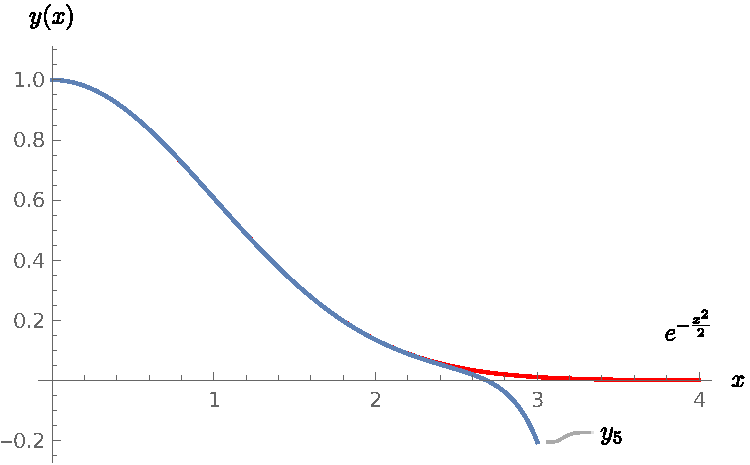
\includegraphics{img/exp_reseni.pdf}
    \caption{Srovnání přesného řešení a páté iterace $y_5$.}
\end{figure}




\subsection{Základní pojmy spektrální analýzy}

Budeme zkoumat operátorovou rovnici pro neznámé $x\in X$
\begin{equation}
    ( \map T -\lambda \Id)x=u\quad,\lambda\in \C,\;  \map T \in \mathscr{L}(x),\;u\in X \text{ Banachův prostor}
    \label{eq:zadani_vlCisla}
\end{equation}
Motivací k tomu je předchozí paragraf. Označme $ \map T_\lambda\coloneqq  \map T -\lambda\Id$, pak $ \map T_\lambda\in \mathscr{L}(X)\Leftrightarrow  \map T \in \mathscr{L}(X)$.

Označme obor hodnot (range) operátoru $ \map T_\lambda$
$$ \mathcal{R}( \map T_\lambda)\coloneqq \{y\in X,\; \exists x\in X,\; \map T_\lambda x=y\}\quad (= \map T_\lambda (X)).$$

Otázky řešitelnosti rovnice (\ref{eq:zadani_vlCisla}) lze přeformulovat v řeči operátoru $ \map T_\lambda$ následovně.
\begin{table}[h!]
    \centering
    \begin{tabular}{c|c}
         V řeči rovnic& V řeči operátoru  \\ \hline\hline
         $\exists$ řešení pro libovolnou pravou stranu $u\in X$? & Je $ \map T_\lambda$ \uu{na}, tj je $ \mathcal{R}( \map T_\lambda)=X$?\\ \hline
         Pokud řešení pro dané $u\in X$ existuje, je určeno jednoznačně? & Je $ \map T_\lambda$ \uu{prostý} na $X$?\\ \hline
         Pokud $\forall u \in \mathcal{R}( \map T_\lambda)\exists! x\in X;\;  \map T_\lambda x=u$, \\je toto řešení \uu{stabilní}? (viz porn. níže)& Je-li $ \map T_\lambda$ prostý, je potom $ \map T_\lambda^{-1}$ spojitý na $\mathcal{R}( \map T_\lambda)$?
    \end{tabular}
\end{table}

\Poznamka 

Pod pojmem \uu{stabilní řešení} míníme (zjednodušeně) situaci, kdy v rovnici $ \map T_\lambda x=u$, která má jednoznačně určená řešení pro $\forall u\in \mathcal{U}(u_0)$ platí, že \uv{malé změny $u\in \mathcal{U}(u_0)$} mají za následek \uv{malé změny řešení}. To přesně odpovídá situaci, kdy je inverzní zobrazení $ \map T_\lambda^{-1}$ spojité na $\mathcal{U}(u_0)$. Tato vlastnost je velmi důležitá při hledání přibližného řešení. Při něm často aproximujeme pravou stranu $u$ nějakou \uv{jí blízkou pravou stranou} $\overline{u}$ a doufáme, že i řešení $\overline{x}$, které odpovídá pravé straně $\overline{u}$, bude blízké řešení $x$, odpovídajícímu pravé straně $u$. Pro \uu{nestabilní} operátory to však nemusí být pravda.

\subsubsection{Podívejme se nejprve na situaci pro $\dim X=n\in \N$.}

V konečné dimenzi je $ \map T \in \mathscr{L}(X)\Leftrightarrow \exists$ matice $M\in \mathcal{M}^{n\times m}$ taková, že $ \map T (x)=Mx \;\;\forall x \in X$ (v $X$ volíme jednu pevnou bázi).

Potom platí 
%$$ Tady je někde chyba! Když se spustí, nekompiluje se
%\begin{split}
% \map T  \text{ je prostý } &\Leftrightarrow   \map T  \text{ je \uu{na} } \;\;\Leftrightarrow \;\;\; \underbrace{M \text{ reprezentující  \map T  \text{ je regulární.}}}_{ \Updownarrow}  \\  
% \map T ^{-1} \text{ je prostý } &\Leftrightarrow  \map T ^{-1} \text{ je na} \Leftrightarrow \overbrace{M^{-1} \text{ je regulární a reprezentuje }  \map T ^{-1} }\text{ (tj }  \map T ^{-1} \text{ je lin. )}
%\end{split}
%$$


Protože v konečné dimenzi je každý lineární operátor spojitý, je i $ \map T ^{-1}\in\mathscr{L}(X)$.

V konečné dimenzi tedy platí \uv{všechno nebo nic}, tzn konečně dimenzionální Fredholmova alternativa pro $ \map T \in\mathscr{L}(X);\;\dim X=n$.

platí právě jedna z násludujících situací:
\begin{enumerate}
    \item $ \map T $ je prostý, na a má spojitou inverzi
    \item $ \map T $ není prostý, není na a nemá spojitou inverzi
\end{enumerate}
\uu{V nekonečné dimenzi} není obecně žádný vztah mezi \uu{prostotou} a zobrazením \uu{na}.

\Priklad

Definujme prostor posloupností $l_2$
$$L_2\coloneqq \Big\{ \{x_n\}_{n=1}^\infty,\; x_n\in\C;\;\sum\limits_{n=1}^\infty|x_n|^2<\infty\Big\}$$

Lze ukázat, že $l_2$ s normou $||\{x_n\}||^2_{l_2}\coloneqq \sum_{n=1}^\infty|x_n|^2$ je Banachův prostor (je dokonce Hilbertův, více později). Na $l_2$ definujme dva tzv. \uu{operátory posunu} (\uv{shift operators})
\begin{equation*}
\begin{split}
  A_1&: (x_1,x_2,x_3,\dots)\mapsto (0,x_1,x_2,x_3,\dots)\\
  A_2&: (x_1,x_2,x_3,\dots)\mapsto (x_2,x_3,x_4,\dots).
\end{split}
\end{equation*}

Evidentně
\begin{equation*}
\begin{split}
  ||A_1x||_{l_2}=||x||_{l_2}&\Rightarrow ||A_1||=\sup\limits_{||x||\leq1}||A_1 x||=1\\
  ||A_2x||_{l_2}=||x||_{l_2}&\Rightarrow ||A_2||\leq1,
\end{split}
\end{equation*}
tedy oa jsou omezené, tedy spojité, tedy $A_1,A_2\in \mathscr{L}(L_2)$.

Přitom \begin{itemize}
    \item $A_1$ je \uu{prosté} (různým prvkům přiřadí různé prvky, ale není \uu{na} (nic se nezobrazí např. na $(1,0,0,\dots)$
    \item $A_2$ je \uu{na}, ale \uu{není prostý} (rozmyslete).
\end{itemize}

Nicméně, co se týče \uu{stability}, tak i v nekonečné dimenzi platí tato hluboká věta:
\begin{theorem}
\label{theorem:str23}
$A\in \mathscr{L}(X)$ Banachův, nechť $A$ je \uu{prosté} a \uu{na}. Potom $A^{-1}\in \mathscr{L}(X)$, tj. $A^{-1}$ je spojitý.
\end{theorem}

\begin{proof}
    Tímto se zdá, že problém \uu{stability} řešení je vyřešen: stačí \uu{prostora} a \uu{na}. Ano, pro lineární omezené (tj. spojité operátory tomu tak je. Ale např, pro lineární a nespojité, nebo pro nelineární operátory není situace tak jednoduchá.
\end{proof}

\subsubsection{Možné stavy operátoru}
Buď $ \map T \in\mathscr{L}(X)$, $X$ je Banachův, $\lambda\in\C,\;  \map T_\lambda\coloneqq  \map T -\lambda\Id \in\mathscr{L}(X)$. Pak v závislosti na $\lambda\in\C$ může operátor $ \map T_\lambda$ mít různé vlastnosti z hlediska jeho prostoty, spojitosti inverze a velikosti $\mathcal{R}( \map T_\lambda)$. Následující tabulka shrnuje všechny možnosti, přičemž dvě z nich nemohou nastat: ta, která je vyloučena větou \ref{theorem:str14} (označeno \uv{V1}) a ta, která je vyloučena lemmatem \ref{lemma1}, které zformulujeme a dokážeme za níže (označeno \uv{L1}).

Tabulku je nutno chápat tak, že pomocí ní definujeme různé kategorie, do kterých může patřit parametr $\lambda\in\C$. Tedy např. levý horní roh tabulky je nutno číst takto: \uv{$\lambda\in\C$ je regulárním bodem $ \map T $, pokud $ \map T_\lambda$ je prosté, $ \map T_\lambda^{-1} $ spojité a $\mathcal{R}( \map T_\lambda)=X$}.

\begin{table}[h!]
    \centering
    \begin{tabular}{c||c|c|c}
         & $\overbrace{\mathcal{R}( \map T_\lambda)=X}^{ \map T_\lambda \text{ je \uv{na}}}$   &  $\overbrace{\mathcal{R}( \map T_\lambda)\neq X,\; \overline{\mathcal{R}( \map T_\lambda)}=X}^{ \map T_\lambda \text{ není \uv{na} }}$ &  $\overbrace{\overline{\mathcal{R}( \map T_\lambda)}\neq X}^{ \map T_\lambda \text{ není \uv{na} }}$ \\ \hline\hline
         $ \map T_\lambda \text{ prostý} \big\{ \exists  \map T_\lambda^{-1}$ a je spojitý & $\lambda$ je regulární bod $ \map T $ &  \diagbox{$L1$} &$\lambda\in\Sp_R( \map T )$ \\ \hline
         $ \map T_\lambda \text{ prostý}\big\{\exists  \map T_\lambda^{-1}$ a není spoj. & \diagbox{$V1$} &  $\lambda\in \Sp_C( \map T )$ &$\lambda\in\Sp_R( \map T )$  \\ \hline
         $ \map T_\lambda \text{ není prostý}\big\{\nexists  \map T_\lambda^{-1}$ & $\lambda\in\Sp_P( \map T )$ &  $\lambda\in\Sp_P( \map T )$ &$\lambda\in\Sp_P( \map T )$  \\
    \end{tabular}
    \caption{Caption}
    \label{tab:spektra}
\end{table}

\uu{Komentář:}
\begin{itemize}
    \item $\Sp_C(\map T)$ \dots tzv. \uu{spojité spektrum} operátoru $ \map T $. Pokud $\lambda\in \Sp_C(\map T)$, tak rovnice $\map T_\lambda y=u$ nemá řešení pro každou pravou stranu $u\in X$ a každému $\epsilon>0$ existuje $u_\epsilon\in X$, $||u_epsilon-u||_X<\epsilon$ a přitom existuje řešení rovnice $\map T_\lambda y=u_\epsilon\in X$ (to je důsledek toho, že $\overline{\mathcal{R}( \map T_\lambda)}=X$). Někdy se jim říká \uv{skorořešení}. Zároveň však $ \map T_\lambda$ je nestabilní ($ \map T_\lambda^{-1}$ je nespojitý), takže nedává dobrý smysl se bavit o tom, co se děje s řešeními, když trochu měníme pravé strany $u_\epsilon$.
    \item $\Sp_R( \map T )$ \dots tzv. \uu{reziduální spektrum}  $\map T$ . Protože $\overline{\mathcal{R}(\map T_\lambda)}\neq X$, nejsou k dispozici řešení pro velkou část $u\in X$
    \item $\S_P$ \dots tzv. \uu{bodové spektrum} $ \map T $. $ \map T_\lambda$ není prostý, tj. 
    $$\exists x_1\neq x_2,\;  \map T_\lambda x_1= \map T_\lambda x_2 $$
    def. $x\coloneqq x_1-x_2\neq 0$, tj. $\exists x\neq 0$ tak, že 
    \begin{equation*}
    \begin{split}
        \map T_\lambda x &=0 \\
        (\map T -\lambda\Id)x&=0\\
        \map T x&=\lambda x.
    \end{split} 
    \end{equation*}
    
\end{itemize}

Tedy $\lambda\in\Sp_P(\map T) \Leftrightarrow \exists x\neq 0:\; \map Tx = \lambda x \xLeftrightarrow{\text{def.}} \uu{\lambda\text{ je vlastní číslo }T}$ a $x\neq0$ je odpovídající vl. vektor.

\begin{definition}[Spektrum operátoru]
Nechť $X$ je Banachův prostor a $\map T \in \lin(X)$. Množinu $$ \map T\in\mathscr{L}(X)$ je $\Sp(\map T)\coloneqq \Sp_C(\map T)\cup \Sp_R(\map T) \cup \Sp_P(\map T)$$ nazýváme spektrem operátoru $\map T$.
\end{definition}


\uu{Pozorování:}
\begin{itemize}
    \item $\lambda\in \Sp(\map T)\Leftrightarrow \map T_\lambda$ není prostý nebo není na
    \item $\lambda$ regulární $\Leftrightarrow \map T_\lambda$ prostý, na (a pak už $\map T_\lambda^{-1}$ spojitý
    \item Ne každý prvek spektra $T$ je vlastním číslem.
\end{itemize}

\begin{definition}[Spektrální poloměr]
Nechť $X$ je Banachův prostor a $\map T \in \lin(X)$. Spektrální poloměr operátoru $\map T$ definujeme předpisem $$ \rho(\map T)\coloneqq \sup \left \lbrace |\lambda|;\; \lambda\in\Sp(\map T) \right \rbrace \:.$$
\end{definition}

\uu{Pozorování:} Pokud je $\rho(\map T) <\infty$, pak platí $|\lambda|>\rho(\map T)\Rightarrow \lambda$ regulární.

Konečně se dostáváme ke slíbenému lemmatu ze spektrální tabulky.
\lemma
$X$ Banachův prostor, $\map A\in\mathscr{L}(X)$. Potom 
\begin{equation*}
    \begin{split}
        \left.
    \begin{array}{ll}
        \mathcal{R}(\map A)\neq X,\; \overline{\mathcal{R}(\map A)}=X & \\
        \exists \map A^{-1}: \mathcal{R}(\map A) \rightarrow X \text{ (tj. }\map A \text{ je prostý)}& 
    \end{array}
        \right \}=\map A^{-1} \text{ není spojitý}.
    \end{split}
\end{equation*}

\begin{proof}
    Nechť $\map A^{-1}$ je spojitý na $\mathcal{R}(\map A)$
    \begin{itemize}
        \item $\mathcal{R}(\map A) \neq X \Rightarrow \uu{\exists y\in X\backslash \mathcal{R}(\map A)}$
        \item $\overline{\mathcal{R}(\map A)}=X \Rightarrow \exists y_n\in\mathcal{R}(\map A);\; y_n\rightarrow y$ v $X$.
        \item $y_n\in\mathcal{R}(\map A) \Rightarrow \exists x_n\in X, \;\map A(x_n)=y_n \Rightarrow x_n=\map A^{-1}(y_n)$
        \item $y_n\in\mathcal{R}(\map A)\Rightarrow \exists x_n\in X,\; \map A(x_n)=y_n \Rightarrow x_n=\map A^{-1}(y_n)$
        \item $y_n$ konverguje v $X \Rightarrow y_n$ je Cauchyovská v $X \xRightarrow{A^{-1} \text{ spoj.}} x_n \text{ je Cauchyovská v } X \xRightarrow{X \text{ úplný}} \exists x\in X$, že  $x_n\rightarrow x$.
        \item Potom ale $\map Ax=A(\lim\limits_{n\rightarrow \infty} x_n)\overset{\map A \text{ spoj.}}{=} \lim\limits_{n\rightarrow \infty} \underbrace{\map Ax_n}_{y_n} =y$
    \end{itemize}
Protože $\exists x\in X,\; \map Ax=y$, je $y\in\mathcal{R}(\map A)$, což je spor s prvním (podtrženým) bodem.
\end{proof}

\begin{remark}[Tabulka \ref{tab:spektra} v konečné dimenzi]

Víme, že $\map T\in \mathscr{L}(X);\; \dim X=n\in \N$ je reprezentován maticí $M\in \mathcal{M}^{n\times n}$.

Potom platí:
\begin{equation*}
\begin{split}
    \map T \text{ je prostý }&\Leftrightarrow \map T \text{ je \uu{na} }\quad \Leftrightarrow\quad \;\; \underbrace{M \text{ je regulární}}_{\Updownarrow} \text{ a reprodukuje } \map T \\
   \map T^{-1}\text{ je prostý }&\Leftrightarrow \map T^{-1} \text{ je na }\Leftrightarrow M^{-1} \overbrace{\text{ je regulární}} \text{ a reprezentuje }\map T^{-1}
\end{split}
\end{equation*} 
Za výše popsané situace je navíc vždy i $\map T^{-1}\in\mathscr{L}(X)$.

Tabulku \ref{tab:spektra} tedy lze schematicky upravit do tvaru
\begin{table}[h!]
    \centering
    \begin{tabular}{c||c|c|c}
    & & & \\\hline\hline
        & \circled{1}& \circled{2},\circled{3} & \circled{4} \\ \hline
        & \circled{2}&\circled{3},\circled{4} & \circled{4} \\ \hline
        & \circled{4}& \circled{3} & \circled{1}
    \end{tabular}
    \caption{Tabulka \ref{tab:spektra} přepsaná v konečné dimenzi}
    \label{tab:spektra_konecnaDim}
\end{table}

\begin{enumerate}[label=\protect\circled{\arabic*}]
\item V \uu{konečné dimenzi} nastává pouze tato situace, a tedy zde máme              
    \begin{enumerate}[label=\arabic*.]
        \item $\lambda\in\C\rightarrow \lambda$ je buď regulární nebo už je to vl. číslo
        \item $\Sp(\map T)=\{ \lambda\in\C,\lambda$ je vlastní číslo $\map T\}=\{\lambda\in\C;\;\lambda$ je vl. číslo $M \}$.
    \end{enumerate}
\item Nemůže obecně nastat
\item Tento sloupec popisuje situaci $\mathcal{R}(\map T_\lambda)\neq X,\; \overline{\mathcal{R}(\map T_\lambda)}=X$. Ta však v konečné dimenzi nastat nemůže, protože v ní platí $\mathcal{R}(\map T_\lambda) = \overline{\mathcal{R}(\map T_\lambda)}$
\item Fourth item
\end{enumerate}

\end{remark}

Následující věta ukazuje, že $\rho(\map T)$ je pro $\map T \in \mathscr{L}(X)$ vždy konečný.
\begin{theorem}
\label{theorem:str26}
    $X$ Banachův, $T\in \mathscr{L}(X)$ (tj. $||T||<\infty$). Potom pro $|\lambda|>||\map T||$ platí

\begin{align*}
        &\circled{A}:\;\; \lambda \in \Sp(\map T)\text{, tj. } \lambda \text{ je regulární}  \\
        &\circled{B}:\;\; (T-\lambda\Id)^{-1}=T_\lambda^{-1}=-\sum\limits_{k=0}^\infty\frac{T^k}{\lambda^{k+1}}\in\mathscr{L}(X) 
\end{align*}
\end{theorem}

\Poznamka \begin{itemize}
    \item Z \circled{A} ihned plyne $\rho(\map T) \leq ||T||$.
    \item Řada v \circled{B} se nazývá von Neumannova řada operátoru $\map T-\lambda \Id)$
\end{itemize}
\begin{proof}
    Je-li $|\lambda|>||\map T||$, pak ještě $\lambda\neq0$. Položme $\map A\coloneqq\frac{1}{\lambda}\map T$. Potom $||\map A||=\frac{1}{|\lambda|}||\map T||<1$ a na $\map A$ můžeme použít větu \ref{theorem:str14}. To nám dá, že:
    \begin{enumerate}[label*=.]
        \item[\circled{A}] $\Id-\map A$ je prostý a na $\Rightarrow \map T-\lambda\Id=(-\lambda)(\Id-\map A$ je prostý a na $\xRightarrow{\text{ věta \ref{theorem:str14}}} (\map T-\lambda\Id )^{-1}$ je spojitý. Odtud je $\lambda$ regulární atd.
        \item[\circled{B}] Věta \ref{theorem:str14} dá i 
        \begin{align*}
            (\Id-\map A)^{-1}&=\sum\limits_{k=0}^\infty \map A^k\\
            (\Id-\frac{1}{\lambda}\T)^{-1}&=\sum\limits_{k=0}^\infty\frac{\map T^k}{\lambda^k} \Big/ \cdot (-1)\\
            \left(\frac{1}{\lambda}\map T-\Id \right)^{-1}&=-\sum\limits_{k=0}^\infty\frac{\map T^k}{\lambda^k} \Big/\cdot \frac{1}{\lambda} \quad pozor!\footnotemark\\
            \underbrace{\lambda^{-1}\left(\frac{1}{\lambda}\map T-\Id \right)^{-1}}_{(\map T-\lambda \Id)^{-1}}&=-\sum\limits_{k=0}^\infty\frac{T^k}{\lambda^{k+1}}
        \end{align*}
      \end{enumerate}
    \footnotetext{Inverzní zobrazení k y=3x je y=x/3, tedy inverzní robrazení má hodnotu koeficientu převrácenou. Na levé straně rovnosti lze tedy (alternativně) postupovat:
           $$ \left(\frac{1}{\lambda} \map T-\Id\right)^{-1}=\lambda (T-\lambda\Id)^{-1}, $$
           a pak je jasné, proč musíme rovnici dělit \lambda.}
\end{proof}

\Priklad 
Uvažujme $l_2\coloneqq \left \{ \{x_n\}_{n=1}^\infty,\; x_n\in\C,\;\sum\limits_{n=1}^\infty|x_n|^2<\infty \right \}$ prostor všech komplexních posloupností, které jsou tzv. \uv{sčítatelné s kvadrátem}. Platí, že $l_2$ se skalárním součinem $\innerprod{\{x_n\}}{\{y_n}\}_{l_2}=\sum\limits_{n=1}^\infty x_n\conj{y_n}$ (který indukuje normu $||\{x_n\}_{l_2}=\sqrt{\sum_{n=1}^\infty}|x_n|^2$) je úplný, a tedy Hilbertův (tj. i Banachův) prostor.

Uvažujme operátor 
\begin{align*}
    \map T&:l_2\rightarrow l_2\\
    \map T&:(x_1,x_2\dots,x_k,x_{k+1},\dots)\mapsto (0,x_1,x_2,\dots,x_{k-1},x_k,\dots).
\end{align*}
Protože $||\map T x ||_{l_2}=||x||_{l_2}$, je $||\map T||=\sup$




\pagebreak
\section{Kompaktní operátory}

Z minulých kapitol víme, že pro \emph{lineární} operátor mezi Banachovými prostory $\map T: X \to Y$ platí: 
$$\map T \text{ je spojitý}\;\Leftrightarrow\;\map T \text{ je omezený},$$
píšeme $\map T\in \lin(X,Y)$. Dále budeme využívat definice $\lin(X)\coloneqq \lin(X,X)$. 

Připomeňme, že $\map T(\text{omezená množina})=\text{omez. množina}$. Tento výrok tedy pro lineární operátory charakterizuje spojitost, jinými slovy $\forall A\subset{X}$ omezená, je $\map T(A)$ omezená v $Y$.

\begin{definition}[Kompaktní operátor]
Nechť $X,Y$ jsou Banachovy prostory, $\map K: X \to Y$ je lineární operátor. Řekneme, že $\map K$ je kompaktní, jestliže pro každou omezenou množinu $A \subset X$ platí, že $\overline{\map K(A)} \subset Y$ je kompatkní množina. Množinu všech kompaktních operátorů zapisujeme jako $\comp(X,Y)$ a zavádíme $\comp(X) \coloneqq \comp(X,X)$.
\end{definition}

\begin{remark}\qquad
\begin{enumerate}
    \item $\comp(X,Y) \subset \lin(X,Y)$. Je-li totiž $A \subset X$ omezená, pak $\overline{\map K(A)} \subset Y$ je kompaktní a podle nutné podmínky kompaktnosti musí být $\overline{\map K(A)} $ omezená a uzavřená množina, tedy i $\overline{\map K(A)}\supseteq \map K(A)$ je omezená.
    \item Připomeňme, že omezenost a uzavřenost jsou postačující podmínky pro kompaktnost pouze v konečnědimenzionálním normovaném lineárním prostoru (NLP).
    \item Pro kompaktní množiny můžeme používat Weierstrassovské vybírání podposloupností, čehož dále využijeme.
\end{enumerate}
\end{remark}

\subsubsection{Charakterizace operátoru pomocí posloupností}
Pro $\map T\in \lin(X,Y)$ jsme měli:
$$\begin{array}{l}
     \text{spojitost: }x_n\rightarrow x\;\Rightarrow \; \map Tx_n\rightarrow \map Tx\\
\text{omezenost: }\{x_n\}\text{ je omezená}\;\Rightarrow \;\{\map T x_n\} \text{ je omezená}
\end{array}$$ 
Charakterizaci kompaktnosti raději shrneme do věty.

\begin{theorem}[O charakterizaci kompaktního operátoru pomocí posloupnosti]
Operátor $\map K :X \to Y$ je kompaktní právě tehdy, když pro každou omezenou posloupnost $\sequence {x_n}{n} \subset X$ existuje vybraná podposloupnost $\sequence{x_{n_k}}{k} $ a prvek $y \in Y$ takový, že $\map K ( x_{n_k}) \rightarrow y $.
\end{theorem}

\begin{proof}[Úkaz:]\qquad

Pokud by celý prostor $Y$ měl vlastnost, že z každé omezené posloupnosti v $Y$ se dá vybrat konvergentní podposloupnost, pak by platilo \begin{align*}
    \lin(X,Y) = \comp (X,Y) \:.
\end{align*}
Tuto úvahu zdůvodníme následovně. Stačí ukázat, že 
\begin{align*}
    \lin(X,Y) \subset \comp (X,Y) \:,
\end{align*}
opačnou implikaci jsme již vyřešili. Buď tedy $\map T \in \lin(X,Y)$ a $\sequence{x_n}{n} \subset X$ omezená posloupnost.
Díky spojitosti $\map T$ je posloupnost $ \sequence{ \map T x_n}{n}$ omezená. Pokud bychom zaručili, že z každé takové posloupnosti už můžeme vybrat konvergentní podposloupnost, dokázali bychom tím kompaktnost každého spojitého operátoru. Takovou vlastnost jistě nemůže mít každý metrický prostor. Na počest Bolzanovy-Weierstrassovy věty platné v $\R$ ji nazveme \emph{B-W vlastností}.
\end{proof}

\begin{lemma}[O nutné podmínce pro B-W vlastnost]
Nechť $Y$ je Banachův prostor. Pak 
$$Y\text{ má B-W vlastnost}\;\Leftrightarrow\;\dim Y<\infty.$$
\end{lemma}

\begin{proof}[Úkaz:]\qquad

\uv{$\Leftarrow$} Na $\R$ můžeme používat Bolzanovu-Weierstrassovu větu z prvního semestru. V prostoru $\R^n$ provedeme postupné výběry po složkách. Nyní jelikož $\dim X=n \in\N$, můžeme najít bázi a každému prvku $x \in X$ přiřadit $n$-tici souřadnic vzhledem k této bázi. 

\uv{$\Rightarrow$} Je-li $\dim Y=\infty$, zvolíme $y_1 \in Y$ a poté indukcí vybíráme prvky $y_{k+1} \in Y$ tak, aby vzdálenost prvku $y_{k+1}$ od prvku $y_k$ byla větší nebo rovna jedné. Po přechodu k libovolné posloupnosti dostaneme stále posloupnost, která má prvky vzdálené od sebe více než o jedničku a proto nemůže splňovat B-C podmínku.
\end{proof}

\begin{lemma}[O kompaktnosti identity] \label{3.kompaktnost identity}
Pro Banachův prostor $X$ v dané normě platí:
$$\map{Id} : X \to X \text{ je kompaktní}\;\Leftrightarrow\;X \text{ má B-W vlastnost}.$$
\end{lemma}
\begin{proof}
Zřejmé.
\end{proof}

Z předchozích dvou lemmat plyne zajímavé zjištění, že \uu{v nekonečné dimenzi není identita kompaktní operátor}. Obecně tedy máme:
$$\map{\Id}\in\lin(X) \text{ je kompaktní }\Leftrightarrow\;\; \dim X<\infty.$$


\begin{remark}
V teorii parciálních diferenciálních rovnic se uplatňuje proces \uv{kompaktního vnoření} jednoho prostoru do druhého. V uvedené situaci uvažujeme dva prostory $ X \subset Y$, ovšem opatřené různými normami $\norm{\cdot}_X, \norm{\cdot}_Y$. Zobrazení $\map{\Id} : X \to Y$ v takovém případě může být kompaktní. Je to ovšem způsobeno právě růzností norem, které na nekonečnědimenzionálních prostorech nejsou ekvivalentní.

Příkladem takového procesu může být tzv. Rellichova věta:

Nechť $\Omega \subset \R^n$ je otevřená omezená množina s hladkou hranicí. Definujme Sobolevův prostor \begin{align*}
    W^{1,2}(\Omega) := \left \lbrace f: \Omega \to \R : \norm{f}_{W^{1,2}} := \left[ \int_\Omega \left( |f|^2 + |\nabla f|^2 \right) \d x \right]^{1/2} < + \infty \right \rbrace \:.
\end{align*}
Pak je $W^{1,2}(\Omega) \subset L^2(\Omega)$ a navíc $\map{\Id} : W^{1,2}(\Omega) \to L^2(\Omega)$ je kompaktní operátor.

Praktické použití této věty spočívá právě ve vybírání konvergentní podposloupnosti v $L^2$ z omezené posloupnosti v~prostoru $W^{1,2}$.
\end{remark}

\subsection{Vlastnosti kompaktních operátorů}
V této podkapitole formulujeme sedm klíčových vlastností, které značně zjednodušují problematiku spektrální analýzy pro kompaktní operátory.

\begin{lemma}
    $\dim Y<\infty \;\Rightarrow\; \lin(X,Y)=\comp(X,Y)$
\end{lemma}
\begin{proof}
$A\subset X$ je omezená$\;\xRightarrow{\map T\in \lin(X,Y)}\;\map T(A)$ je omezená$\;\Rightarrow\; \overline{\map T(A)}$ je omezená a uzavřená v $Y\;\xRightarrow{\dim Y<\infty} \; \overline{\map T(A)}$ je kompaktní.
\end{proof}

Důsledkem tohoto lemmatu je $T\in\lin(X),\;\dim X=\infty,\;\dim \mathcal{R}(T)<\infty\;\Rightarrow T\in\comp(X)$.

\begin{lemma}\label{3.skladani}
$\map S \in \lin (X)$, $\map K \in \comp{(X)} \;\Rightarrow \map S \circ \map K\in\comp {(X)}$, $\map K \circ \map S\in\comp{(X)}$.
\end{lemma}

\begin{proof}
Zvolme omezenou posloupnost $\sequence{x_n}{n} \subset X$. Pak $\sequence{\map S x_n}{n}$ je omezená a díky kompaktnosti $\map K$ můžeme z~posloupnosti $\sequence{(\map K \circ \map S) x_n}{n}$ vybrat konvergentní podposloupnost, proto je $\map K \circ \map S$ kompaktní. Dále, z~posloupnosti $\sequence{\map K x_n}{n}$ můžeme vybrat konvergentní $\sequence{\map K x_{n_k}}{k}$ a díky spojitosti operátoru $\map S$ je i~podposloupnost $\sequence{(\map S \circ \map K) x_{n_k}}{k}$ konvergentní, proto je $\map S \circ \map K$ kompaktní.

\end{proof}

\begin{lemma}%[O příslušnosti nuly do spektra kompaktního operátoru]
$\map K\in\comp(X)\; \dim X=\infty \;\Rightarrow 0\in\Sp(\map K)$
\end{lemma}

\begin{proof}
$0\notin\Sp(\map K) \;\Rightarrow \exists \map K^{-1} \in \lin(X)$. Pak dle Lemmatu \ref{3.skladani} dostáváme, že 
$$\underset{\in \comp}{\map K} \circ \underset{\in \lin}{\map K^{-1}} \underset{\Rightarrow}{=} \underset{\in \comp}{\map{\Id}},$$
přičemž kompaktnost identity je ve sporu s Lemmatem \ref{3.kompaktnost identity}.
\end{proof}

\begin{lemma}%[O uzavřenosti obrazu kompaktního operátoru a Fredholmova alternativa]
$\map K \in \comp(X),\; \lambda \neq 0$. Pak 
\begin{enumerate}
    \item $\mathcal{R}(\map K - \lambda \map{\Id})$ je uzavřená množina. (viz \textsc{Lukeš 5.17})
    \item $\map K$ je na (tj. $\mathcal{R}(\map K - \lambda \map{Id} )=X$) $\Leftrightarrow \map K - \lambda \map{\Id}$ je prostý (viz Lukež 5.27).
\end{enumerate}
\end{lemma}
\begin{remark}
Druhé části předchozího lemmatu se říká \uv{Fredholmova alternativa v nekonečné dimenzi}.
\end{remark}

Pro  $\map K\in \comp(X)$, $\lambda\neq 0$ můžeme na základě nově nabytých znalostí upravit spektrální tabulku. Konkrétně jsme zjistili, že
\begin{enumerate}
    \item[a)] nemůže nastat situace $\mathcal{R}(\map K_\lambda)$ a $\overline{\mathcal{R}(\map K_\lambda)}=X$
    \item[b)] $\map K_\lambda$ je prostý $\Leftrightarrow \;\map K_\lambda$ je na.
\end{enumerate}
Máme tedy

\begin{table}[h!]
    \centering
    \begin{tabu}{c||c|c|c}
  &$\mathcal{R}(\map K_\lambda)=X$ & $\mathcal{R}(\map K_\lambda)\neq X$, $\overline{\mathcal{R}(\map K_\lambda)}=X$     &  $\overline{\mathcal{R}(\map K_\lambda)}\neq X$ \\\hline\hline
  
  $\map K_\lambda$ je prostý, $\map K_\lambda^{-1}$ je spojitý     & $\lambda$ je regulární & \strike{|[0pt]c|}{}  & \strike{|[0pt]c|}{b)} \\\hline 
  
  $\map K_\lambda$ je prostý, $\map K_\lambda^{-1}$ není spojitý    & \strike{|[0pt]c|}{}     & \strike{|[0pt]c|}{}   & \strike{|[0pt]c|}{b)}\\ \hline
   
   $\map K_\lambda$ není prostý  & \strike{|[0pt]c|}{b)} & \strike{|[0pt]c|}{a)} & $\lambda\in \SpP$ (je vl. číslo) 
    \end{tabu}
\end{table}

\uu{Shrnutí:}
\begin{itemize}
    \item $0$ je vždy ve spektru kompaktního operátoru. Je jediným prvkem spektra, který nemusí být vlastním číslem.
    \item Všechny nenulové prvky spektra už jsou vlastní čísla.
\end{itemize}


\begin{lemma}%[O nenulových prvcích spektra kompaktního operátoru]
$\map K \in \comp(X)$, $\lambda \neq 0\in \Sp(\map K)$. Pak \begin{itemize}
    \item $\lambda$ je vlastní číslo,
    \item $\dim(\map K - \lambda \map{\Id} ) < + \infty$,
    \item $\Ker (\map K - \lambda \map{\Id} )$ je prostor všech vl. vektorů příslušných vl. číslu $\lambda$ a je uzavřeným podprostorem $X$.
\end{itemize}
\end{lemma}

\begin{proof}
viz. \textsc{Lukeš 5.15}
\end{proof}

\begin{definition}[Násobnost vlastního čísla]
Číslo $\dim \, \Ker (\map K - \lambda \map{\Id} )\in\N$ nazýváme násobností vlastního čísla $\lambda\in\SpP(\map K)$.
\end{definition}

Dle předchozího lemmatu víme, že \uu{každé nenulové vlastní číslo má konečnou násobnost} - dimenze prostoru generovaného vlastními vektory, příslušejících jednomu nenulovému vlastnímu číslu, je konečná.

\begin{lemma}%[O hromadných bodech spektra kompaktního operátoru]
$\map K \in \comp(X)$. Pak $\forall\varepsilon>0$ je množina 
    $\Sp(\map K) \cap \left \lbrace \lambda \in \C : |\lambda| > \varepsilon \right \rbrace$ konečná.
\end{lemma}
Důsledkem toho je, že spektrum kompaktního operátoru je nejvýše spočetné. Navíc má-li spektrum kompaktního operátoru hromadný bod, pak jím může být pouze $0$.

\begin{lemma}
Mějme posloupnost Banachových prostorů $\{X_n\}_{n=1}^\infty$ takovou, že
\begin{itemize}
    \item $ \dim X_n<\dim X_{n+1}<\infty$ 
    \item $X_n\subset X_{n+1}$.
\end{itemize}
Dále definujme operátor $\map K\in\lin(X,X_n)=\comp(X,X_n),\;\;\map K_n: X\to X_n\subset X$, pro nějž $\exists  \; T\coloneqq \lim\limits_{n\rightarrow \infty} \map K_n$, což je operátor definovaný v $\lin(X)$. Pak je $\map K\in \comp(X)$.

\end{lemma}

\begin{corollary}
Pro platnost tohoto lemmatu není podstatné, zda $\lim X_n= X$, či $\lim X_n\neq X$.
\end{corollary}


\pagebreak

%
%Několik poznámek ke značení:
%Pro přehlednost jsem se snažil psát u symbolu normy a skalárního součinu, v jakém prostoru se vlastně norma tvoří. Při učení několika dlouhých operátorových nerovností mi tato drobnost pomohla.
%Rozhodl jsem se rovněž označit nějakým způsobem lineární operátory a zobrazení. Symbol \lin používám pro označení prostoru spojitých lineárních zobrazení a samotná je označuji \map.
%V kapitole duální operátor se ovšem těžko rozlišuje mezi prvky prostoru a jeho duálu. Značení ponechávám, ale lze ho kdykoli vylepšit nebo tak něco.
%Při psaní se držím souboru s originálními poznámkami, ale také svých vlastních poznámek. Některé rozčlenění tyou "Poznámka vs Příklad vs Hlavní text" jsem trochu přizpůsobil k svému obrazu, snad to není na škodu.





\section{Duálnost}

\subsection{Duál a dualita}

\begin{definition}[Duál]
Buď $X$ Banachův prostor. Prostor $X' \coloneqq \lin(X,\C)$ \hspace{0.5em} (resp. $\lin(X, \R)$) nazýváme topologickým duálem k $X$.
\end{definition}

\begin{remark} \ph{.}
\begin{itemize}
    \item Prostor $X'$ je tedy tvořen všemi spojitými lineárními funkcionály, spojitost uvažujeme ve smyslu \begin{align*}
        x_n \xrightarrow{X} x \implies \map T x_n \to \map T x \quad \text{pro všechna } \map T \in X' \:.
    \end{align*}
    \item Víme, že jsou-li $X,Y$ normované prostory a $Y$ je Banachův, pak i $\lin (X,Y)$ je Banachův. Proto je $X'$ automaticky Banachovým prostorem.
    \item Je-li $\map T \in X'$, pak jeho norma je přirozeně $\norm{\map T}_{X'} := \underset{\norm{x}_X \leq 1}{\sup} |\map Tx|$.
    \item Topologický duál není totéž, co \uu{vektorový duál} (pouze lineární zobrazení $X \to \C$ ($\R$), nevyžaduje spojitost). Prvků vektorového duálu je víc (o ony „nespojité“). V konečné dimenzi pro $X$ Banachův je vektorový duál vždy topologickým duálem.
\end{itemize}
\end{remark}


\begin{definition}[Dualita]
Nechť $X$ je Banachův a $X'$ jeho duál. Zobrazení $\map S : X \times X' \mapsto \C$ nazveme dualitou, jestliže splňuje vlastnosti: \begin{enumerate}
    \item sekvilinearita: $\map S(\alpha x + \beta y, z) = \alpha \map S(x,z) + \beta \map S(y,z), \;\; \map S(z,\alpha x + \beta y) = \conj{\alpha} \map S(z,x) + \conj{\beta} \map S(z,y)$.
    
    \item spojitost: $\map S(x_n,y_n) \rightarrow \map S(x,y) \quad \text{kdykoliv } (x_n,y_n) \rightarrow (x,y) \text{ v } X \times X'$.
\end{enumerate}
Někdy píšeme $\map S(x, \map T) = \duality{x}{\map T}$. Obecně je často $\duality{\cdot}{\cdot}$ symbolem duality.
\end{definition}

\begin{remark}
Jsme-li v nějakém smyslu schopni ztotožnit prostory $X$ a $X'$ (uvidíme v následujícím), pak roli duality hraje skalární součin. Ztotožněním prostorů myslíme následující: píšeme $X \simeq Y$, jestliže existuje zobrazení $\map D: X \mapsto Y$, které je izometrické a izomorfní, tj. zachovává normu a je bijektivní.
\end{remark}

\begin{example}

Uvažujme prostor vektorů $\R^n$. Víme, že každá lineární forma $\map T \in {\R^n}'$ je reprezentovatelná lineární kombinací (násobení transponovaným vektorem): $\map T \left[ (x_1, \cdots, x_n) \right] = \sum_{j=1}^n \alpha_j x_j$. Transponování je izometrické a izomorfní zobrazení, lze tedy psát $\R^n \simeq {\R^n}'$. Dualitou na takovém prostoru je například \textit{skalární součin} na $\R^n$. Později uvidíme, že podobně lze uvažovat i v jakémkoliv Hilbertově prostoru – v tomto smyslu je dualita zobecněním skalárního součinu.
\end{example}

\begin{theorem}[O ztotožnění sdružených Lebesgueových prostorů]
Buď $\Omega \subseteq \R^n $ otevřená souvislá množina, $\map T \in L^q(\Omega)'$. Nechť pro $p \in (1, \infty)$ platí $\frac{1}{p} + \frac{1}{q} =1$ ($p$ je tzv. sdružený exponent ke $q$). Pak existuje právě jeden prvek $g \in L^p(\Omega)$ takový,~že:
$$
\map T(f) = \int_\Omega f \conj{g} \d x \quad \forall f \in L^p(\Omega)
\quad \text{a zároveň} \quad
\norm{\map T}_{L^p(\Omega)'} = \norm{g}_{L^q(\Omega)} \:.
$$

\end{theorem}

\begin{proof}
Dokázat, že takové zobrazení existuje, nedá příliš práce. Dokázat jeho jednoznačnost je však velmi pracná záležitost.
\end{proof}

Předchozí věta ukazuje, že platí $L^p(\Omega)' \simeq L^q(\Omega)$. V tomto smyslu ztotožňujeme $\map T$ a $g$, a dualitu $\duality{f}{\map T} \mapsto \map T(f)$ ztotožňujeme s dualitou
\begin{equation}
    \duality{f}{g} \mapsto \int_\Omega f \conj g, \quad f \in L^p, \, g \in L^q \: .
    \label{eq:4.Dualita Lebesgue}
\end{equation}
Povšimněme si, že pokud v předchozí větě položíme $p=q=2$, získáme vlastnost $L^2(\Omega)' \simeq L^2(\Omega)$ a dualita \eqref{eq:4.Dualita Lebesgue} má stejný tvar jako skalární součin na $L^2(\Omega), \; \duality{f}{g} \equiv \innerprod{f}{g}_{L^2}$. Je přirozené se ptát, zda se za tímto výsledkem skrývá něco hlubšího. Odpověď je pozitivní.

\begin{theorem}[Rieszova-Fréchetova o reprezentaci] \label{4.Riesz-Frechet}
Buď $H$ Hilbertův prostor se skalárním součinem $(\cdot \, , \cdot)_H$, $\map T \in H'$.
Pak existuje právě jeden prvek $f \in H $ takový, že plátí následující:
\begin{enumerate}
    \item $\map T(x) = \innerprod{x}{f}_H \quad \text{pro každé } x \in H \:, $
    \item $\norm{\map T}_{H'} = \norm{f}_H \:.$
\end{enumerate}
\end{theorem}
\begin{proof}
viz Lukeš 2.9
\end{proof}

\begin{corollary}
Zobrazení $\map T \mapsto f$ je izometrický izomorfismus (zachovává normu a je bijektivní). Proto pro všechny Hilbertovy prostory $H$ můžeme provést ztotožnění $H' \simeq H$.
\end{corollary}

% ALERT ALERT TOHLE JE V POZNÁMKÁCH ŠPATNĚ
% T(x) BY NEBYLO LINEÁRÍ, ALE ANTILINEÁRNÍ ZOBRAZENÍ
%\begin{remark}
%V prvním tvrzení věty \ref{4.Riesz-Frechet} by mohlo ekvivalentně být $\map T(x) = \innerprod{f}{x}_H$. Skutečně: položme $\map S(x) = \conj{\map T(x)}$, pak podle Riesz-Fréchetovy věty nalezneme $g \in H$ takové, že $\map S(x) = \innerprod{x}{g}_H$. Potom $\map T(x) = \conj{\map S(x)} = \conj{\innerprod{x}{g}} = \innerprod{g}{x}$.
%\end{remark}

\begin{lemma}[O inkluzi duálních prostorů]
    Nechť jsou $X,Y$ Banachovy a platí $X \subset Y$ a $\norm{x}_Y = \norm{x}_X \; \forall x \in X$. Potom platí $Y' \subset X'$ ve smyslu zúžení zobrazení (restrikce). Zde je však důležité dát velký pozor, je snadné tento výsledek špatně interpretovat!
\end{lemma}
\begin{proof}
    \begin{align*}
    \text{Mějme } \map T \in Y'
    &\implies
    \map T \text{ spojité a lineární (na prvcích z $Y$) }
    \\
    &\implies
    \map T|_X \text{ spojité a lineární (na prvcích z $X$)}
    \implies
    \map T|_X \in X'
    \end{align*}
\end{proof}

\begin{example}
Bezhlavá aplikace předchozí inkluze nás může zahnat do slepých ulic.
\\
Uvažujme prostor $\R \subset \R^2$. Dle předchozího tvrzení můžeme prohlásit $(\R^2)' \subset (\R)'$. Protože jsou oba prostory Hilbertovy, lze je ztotožnit $(\R^n)' = \R^n $, proto by mělo platit $\R^2 \subset \R$, což je zřejmě nesmysl. Kde je ale chyba?

\begin{align*}
    \hspace{-3em}
    \R \subset \R^2 \quad \implies \quad
    (\R^2)' &\subset \R' \\[-5pt]
    \mask{(\R^2)'}{\rotatebox[origin=c]{90}{=}} &\ph{\subset} \;\; \mask{\R'}{\rotatebox[origin=c]{90}{=}} \\[-5pt]\mask{(\R^2)'}{\R^2} &\subset \mask{\R'}{\R}
\end{align*}
V předchozích úvahách jsme učinili dvě chyby: jednu větší, ️jednu menší. \begin{enumerate}
    \item Menší chybu jsme učinili tím, že jsme $(\R^n)' \simeq \R^n$ považovali rovnost, ve skutečnosti je to \textit{ztotožnění}. Každé lineární zobrazení na $\R^n$ má tvar $$\map T(x) = \sum_{j=1}^n \alpha_j x_j$$ a ztotožňuje se s $n$-ticí koeficientů $$T \simeq (\alpha_1, \dots \alpha_n) \in \R^n \text{ reprezentuje } (\R^n)' \: .$$ Na ono reprezentující $\R^n$ je tedy třeba nahlížet opravdu jako na prostor prvků, které reprezentují lineární zobrazení.
    \item Velkou chybu jsme učinili, když jsme inkluzi $(\R^2)' \subset \R'$ považovali za množinovou inkluzi. Tvrzení je třeba chápat v tomto smyslu:
    
    \begin{center}
    „Všechna lineární zobrazení pracující na $\R^2$ lze zúžit tak, aby pracovala na $\R$.“
    \end{center}
    
    Pokud je lineární zobrazení $\map T \in (\R^2)'$ reprezentovatelné dvojicí $(\alpha_1, \alpha_2) \in \R^2$, lze toto zobrazení skutečně zúžit na $\map T|_\R$ reprezentované $(\alpha_1, 0)$, který můžeme považovat za prostor $\R$. To je pravý smysl \uv{inkluze} $Y' \subset X'$.
\end{enumerate}
\end{example}

\bigskip

\begin{remark}
\uv{Duálnost} se často projevuje tím, že vzorce obsahující prvky $X$ a $X'$ vykazují jisté symetrie. Například víme, že
$$\norm{\map T}_{X'} = \sup_{\norm{x}_X \leq 1} |\map T(x)|.$$
Dále víme, že $|\map T(x)| \leq \norm{\map T} \norm{x}_X$. 
\end{remark}

Uvažujme nyní funkcionál $\map T \in X'$ takový, že $\norm{\map T}_{X'} \leq 1$. Pak jistě platí $|\map T x| \leq \norm{x}_X$ a po přechodu k supremu i \begin{align*}
    \sup_{\norm{\map T}_{X'} \leq 1} |\map T(x)| \leq \norm{x}_X \:.
\end{align*}
Následující věta ukazuje, že platí dokonce \textit{rovnost}: \begin{align*}
    \sup_{\norm{\map T}_{X'} \leq 1} |\map T(x)| = \norm{x}_X \:.
\end{align*}

\begin{theorem}[Hahnova-Banachova]
Buď $X$ Banachův, $x \in X$ takové, že $x \neq 0$. Pak existuje $\map T \in X'$ s vlastnostmi \begin{align*}
    \map T(x) = \norm{x}_X \:, \qquad \norm{\map T}_{X'} = 1 \:.
\end{align*}
\end{theorem}

\subsection{Duální zobrazení, duální operátor}

\begin{definition}[Duální zobrazení]
Nechť $X,Y$ jsou Banachovy prostory, $\map T \in \lin (X,Y)$, $\map T' : Y' \mapsto X'$. Řekneme, že $\map T'$ je duální zobrazení k $\map T$, jestliže \begin{align*}
    \map T' \circ \map y' = \map y' \circ \map T' \quad \text{pro všechna } \map y' \in Y' \:,
\end{align*}
neboli \begin{align*}
    \underbrace{(\map T' \circ \map y')}_{\in X'} \underbrace{(x)}_{\in X} = \underbrace{\map y'}_{\in Y'} \underbrace{(\map T x)}_{\in Y} \quad \text{pro všechna } \map y' \in Y' \text{ a všechna } x \in X \:.
\end{align*}
\end{definition}

V předchozí definici je klíčové uvědomit si příslušnost jednotlivých objektů. \begin{itemize}
    \item $\map y' \in Y'$ je zobrazení pracující na $Y$,
    \item $\map T' \map y' \in X'$ je zobrazení pracující na $X$,
    \item $(\map T \map y')(x)$ je objekt, který přiřazuje prvkům z $X \times X'$ číslo. To odpovídá struktuře duality.
\end{itemize}
S použitím tzv. \textit{kanonické} duality $\duality{\map F}{g} = \map F(g)$ můžeme zapsat definici duálního zobrazení v symetrickém tvaru:
\begin{align*}
    \duality{\map T' \map y'}{x} = \duality{\map y'}{\map T x} \: .
\end{align*}
Povšimněme si, že na levé straně máme zobrazení $X' \times X \to \C$ a na pravé zobrazení $Y' \times Y \to \C$.

\begin{lemma}
Je-li $\map T \in \lin (X,Y)$, pak i $\map T' \in \lin(Y', X')$. 
\end{lemma}
\begin{proof}
Linearita je zřejmá. Ukažme spojitost.  Zafixujme $\sequence{\map y'_n}{n} \subset Y'$ takovou, že $\map y'_n \rightarrow \map y'$. Ukážeme, že posloupnost $\sequence{\map T \map y}{n} \subset X'$ konverguje k $\map T \map y_n$. Platí
\begin{align*}
    \norm{\map T' \map y'_n - \map T' \map y'}_{X'} 
    =&
    \sup_{\norm{x} \leq 1} \norm{\map T' \map y'_n (x)- \map T' \map y' (x)}_X 
    =
    \sup_{\norm{x} \leq 1} \norm{\map y'_n  (\map T x)- \map y' (\map T x)}_X 
    =
    \sup_{\norm{x} \leq 1} \norm{(\map y'_n-\map y') (\map T x)}_X 
    \leq \\
    \leq&
     \sup_{\norm{x} \leq 1} \norm{\map y'_n - \map y'} \norm{\map T} \norm{x}
    =
    \norm{\map y'_n -\map y'} \norm{\map T} \rightarrow 0\:,
\end{align*}
což jsme chtěli ukázat.
\end{proof}
\begin{remark}
Dá se ukázat, že: $\map T$ je kompaktní operátor právě tehdy, když je $\map T'$ kompaktní operátor (tzv. Schauderova věta). Sami zkuste dokázat, že $\norm{\map T} = \norm{\map T'}$.
\end{remark}

\bigskip

Dále nás bude zajímat, lze-li ztotožnit $\map T$ a $\map T'$ (podobně jako ztotožňujeme Hilbertův prostor s vlastním duálem). To by znamenalo:
$$
    \underbrace{\map T}_{X \to Y} \;\simeq \underbrace{\map T'}_{Y' \to X'}
$$
Muselo by tedy platit něco ve smyslu
$$ X \simeq Y' \quad \text{a} \quad Y \simeq X' \: , $$
vezmeme-li nyní duál předchozích výrazů, dostaneme
$$ X' \simeq Y'' \quad \text{a} \quad Y' \simeq X'' \: . $$
Zkombinováním obou „rovnic“ získáme s trochou \textit{máchání rukami} výraz
$$ X \simeq X'' \quad \text{a} \quad Y \simeq Y'' \: . $$
To by mohlo platit pro Hilbertovy prostory, kde je dokonce už i $X' \simeq X$. Obecně k danému $\map T$ nemusí vždy existovat $\map T'$, výše uvedené vlastnosti platí pouze v případě, že existuje. Ale v Hilbertově prostoru je opět vše lepší:

\begin{theorem}[O duálním zobrazení mezi Hilbertovými prostory]
Nechť $H_1, H_2$ jsou Hilbertovy prostory a $\map T \in \lin(H_1, H_2)$. Pak existuje právě jedno zobrazení $\map T' : H_2 \mapsto H_1$ takové, že 
\begin{align} \label{eq4.dualHilbert}
    (\map T x, y)_{H_2} = (x, \map T'y)_{H_1} \quad \text{pro všechna } x \in H_1, \; y \in H_2 \:.
\end{align}
Pro takové zobrazení navíc platí: \begin{enumerate}
    \item $\map T' \in \lin(H_2, H_1)$,
    \item $\norm{\map T'} = \norm{\map T \vph{\map T'}}$.
\end{enumerate}
\end{theorem}

\begin{remark}
Aplikujeme-li komplexní sdružení na rovnici \eqref{eq4.dualHilbert}, dostaneme \begin{align*}
    \conj{\innerprod{\map T x}{y}}_{H_2} = \conj{\innerprod{x}{\map T' y}}_{H_1} \rightarrow \innerprod{\map T' y}{x}_{H_1} = \innerprod{y}{\map T x}_{H_2} \:.
\end{align*}
Na Hilbertových prostorech tedy hraje roli duality skalární součin.
\end{remark}
\begin{proof}
Zafixujme $y \in H_2$ a definujme
\begin{gather*}
    \map L_y \in \lin(X, \C) \: ,\\
    \map L_y(x) \coloneqq \innerprod{\map T x}{y}_{H_2} \: .
\end{gather*}
Podle Rieszovy-Fréchetovy věty (Věta \ref{4.Riesz-Frechet}) existuje právě jedno $z \in H_1$ takové, že \begin{align*}
    \map L_y(x) = \innerprod{x}{z}_{H_1} \:.
\end{align*}
Nyní definujeme zobrazení:
\begin{gather*}
    \map T': H_2 \to H_1 \: ,\\
    \map T'(y) \coloneqq  z \: .
\end{gather*}
Toto zobrazení má vlastnost
$$
    (\map T x, y)_{H_2} = (x,\map T' y)_{H_1} \quad \text{pro libovolné } x\in H_1, y \in H_2 \:.
$$
Tím jsme dokázali první část tvrzení o existenci a jednoznačnosti zobrazení $\map T'$.

Ukažme jeho linearitu. Zřejmě je pro každé $x \in H_1$ splněno
\begin{align*}
    \left( \map T' (\alpha y_1 + \beta y_2) , x \right)_{H_1} =& \left( \alpha y_1 + \beta y_2 , \map T x \right)_{H_2} = \alpha (y_1, \map T x)_{H_2} + \beta (y_2, \map T x)_{H_2} = \\
    =&
    \alpha (\map T' y_1, x)_{H_1} + \beta (\map T' y_2, x)_{H_1} = (\alpha \map T' y_1 + \beta \map T' y_2, x)_{H_1}
\end{align*}
a odtud
\begin{align*}
    \map T' (\alpha y_1 + \beta y_2) = \alpha \map T' y_1 + \beta \map T' y_2 \:.
\end{align*}

Ukažme spojitost zobrazení $\map T'$ pomocí omezenosti jeho normy. Podle definice zobrazení $\map T'$ a druhé části Rieszovy-Fréchetovy věty (Věta \ref{4.Riesz-Frechet}) dostáváme \begin{align} \label{eq:4.Vdual1}
    \norm{\map T' y}_{H_1} = \norm{ z}_{H_1} = \norm{\map L_y} \:.
\end{align}
Dále je podle definice $\map L_y$ a Cauchyovy-Schwarzovy nerovnosti \begin{align*}
    \norm{\map L_y x} = |(\map Tx, y)_{H_2}| \leq \norm{\map Tx}_{H_2} \norm{y}_{H_2} \leq \norm{\map T} \norm{x}_{H_1} \norm{y}_{H_2}
\end{align*}
a odtud s použitím \eqref{eq:4.Vdual1} plyne
\begin{align*}
    \norm{\map T' y}_{H_1} = \norm{\map L_y} = \sup_{\norm{x}_{H_1} \leq 1} \norm{\map L_y x}_{H_2} \leq \norm{\map T} \norm{y}_{H_2} \:.
\end{align*}
\begin{align*}
    \norm{\map T'} = \sup_{\norm{y}_Y \leq 1} \norm{\map T' y} \leq  \norm{\map T} \sup_{\norm{y} \leq 1} \norm{y}_{H_2} = \norm{\map T} < + \infty \:.
\end{align*}
Tím jsme ověřili spojitost a celkově $\map T' \in \lin(H_2, H_1)$.

Zbývá ukázat rovnost norem $\norm{\map T'} = \norm{\map T}$. Za tím účelem definujeme $\map T'' = (\map T')'$. O tomto zobrazení již víme, že $\map T'' \in \lin(H_1, H_2)$, $(\map T'' x,y)_{H_2} = (x, \map T' y)_{H_1}$ a $\norm{\map T''} \leq \norm{\map T'}$. Pak s použitím předchozích částí důkazu dostaneme \begin{align*}
    (\map T'' x,y)_{H_2} = (x, \map T'y)_{H_1} = \conj{(\map T' y, x)}_{H_1} = \conj{(y, \map T x)}_{H_2} = (\map T x,y)_{H_2} \quad \text{ pro všechna } x \in H_1, y \in H_2 \:,
\end{align*}
tedy \begin{align*}
    \map T'' x= \map T x \quad \text{pro každé } x \in H_1 \:.
\end{align*}
Odtud \begin{align*}
    \norm{\map T} = \norm{\map T''} \leq \norm{\map T'} \leq \norm{\map T} \:,
\end{align*}
a proto musí platit v předchozím řetězci všude rovnosti.
\end{proof}
\begin{definition}[Hermitovsky sdružený operátor]
Nechť $H_1, H_2$ jsou Hilbertovy prostory, $\map T \in \lin (H_1, H_2) $. Zobrazení $\map T'$ s vlastnostmi z předchozí věty nazýváme hermitovsky sdružený operátor s $\map T$ (případně adjungovaný operátor~k~$\map T$).
\end{definition}

\begin{definition}[Samoadjungovaný (omezený) operátor.]
Nechť $H$ je Hilbertův prostor. Operátor $\map T \in \lin(H)$ nazveme (omezený) samoadjungovaný  (případně hermitovský), jestliže $\map T = \map T'$.
\end{definition}
\begin{remark}
V předchozí definici jsou oba operátory $\map T, \map T'$ definovány na celém Hilbertově prostoru. Zdůrazňujeme zde, že mluvíme o \uv{omezených samoadjungovaných} operátorech. V případě neomezených operátorů uvidíme, že definiční obor operátorů zcela mění spektrální vlastnosti a definice hermitovskosti a samoadjungovanosti je složitější.
\end{remark}

\subsection{Vlastnosti samoadjungovaných operátorů}

\begin{lemma}[O vlastních číslech samoadjungovaných operátorů]
Nechť $\map T \in \lin (H)$ je samoadjungovaný. Pak má pouze reálná vlastní čísla a vlastní vektory příslušející různým vlastním číslům jsou na sebe kolmé.
\end{lemma}
\begin{proof}
První část tvrzení plyne z rovnosti \begin{align*}
\lambda \norm{x}^2_H = (\lambda x, x)_H = (\map T x,x)_H = (x, \map T x)_H = (x, \lambda x)_H = \conj{\lambda} (x,x)_H = \conj{\lambda} \norm{x}_H ^2 \:.
\end{align*}
Nechť jsou $\lambda_1 \neq \lambda_2$ vlastní čísla příslušející vlastním vektorům $y_1,y_2$. Pak z rovnosti \begin{align*}
    (\lambda_1 - \lambda_2)(y_1,y_2)_H = (\lambda_1 y_1,y_2)_H - (y_1, \lambda_2 y_2)_H = (\map T y_1, y_2)_H - (y_1, \map T y_2)_H = (\map T y_1,y_2)_H - (\map T y_1,y_2)_H = 0
\end{align*}
vidíme, že musí platit $(y_1,y_2)=0$.
\end{proof}
\begin{remark}
Samoadjungovaný operátor může mít ovšem i jiné prvky spektra. O nich obecně nevíme nic.
\end{remark}
\begin{theorem}[O spektrálních vlastnostech samoadjungovaných operátorů]
Nechť $H$ je Hilbertův prostor a $\map T \in \lin (H)$ je samoadjungovaný operátor. Označme \begin{align*}
    m(\map T) = \inf \left \lbrace (\map T x,x)_H : \norm{x}_H = 1 \right \rbrace \qquad M(\map T) = \sup \left \lbrace (\map T x,x)_H : \norm{x}_H = 1 \right \rbrace
\end{align*} Pak \begin{enumerate}
    \item Je-li $\lambda \in \sigma(\map T)$, pak $\lambda \in [m(\map T), M(\map T)]$.
    \item Platí $\rho(\map T) = \norm{\map T}$. Speciálně: alespoň jedna z hodnot $\lambda = \pm \norm{\map T}$ je vlastním číslem $\map T$.
\end{enumerate}
\end{theorem} 

\begin{exercise}
Nechť $\mathbb{A} \in \R^{n \times n}$ je reálná symetrická matice, $x \in \R^n$ a $f(x) = (\mathbb{A} x,x) = \sum_{i,j} a_{ij} x_i x_j$. Určete minimum a maximum $f$ za podmínky $\norm{x} =1$.
\end{exercise}

\subsection{Kompaktní samoadjungované operátory na Hilbertových prostorech}

Nejprve zopakujeme výsledky, které zatím máme o kompaktních samoadjungovaných operátorech. Na Hilbertově prostoru $H$ uvažujme $\map K \in \comp (H)$ takový, že $(\map K x,y)_H = (x, \map K y)_H$ pro všechna $x,y \in H$. Pak platí \begin{enumerate}
    \item $\map K$ má nejvýše spočetně mnoho vlastních čísel, všechna vlastní čísla jsou reálná.
    \item Jediným dalším prvkem spektra $\sigma(\map K)$ může být číslo $0$, ta může nebo nemusí být vlastním číslem.
    \item Ke každému nenulovému vlastnímu číslu existuje nejvýše konečně mnoho lineárně nezávislých vlastních vektorů. Navíc vlastní vektory odpovídající různým vlastním číslům jsou na sebe vždy kolmé.
\end{enumerate}

Hlavním výsledkem této kapitoly bude Hilbertova-Schmidtova věta, která říká následující: všechny vlastní vektory odpovídající všem vlastním číslům kompaktního samoadjungovaného operátoru tvoří bázi Hilbertova prostoru. Nejprve je však potřeba provést přípravné práce.

První takovou prací je připomenutí ortogonálního doplňku z lineární algebry.
\begin{definition}[Direktní součet podprostorů]
Nechť $H$ je lineární vektorový prostor a $A,B$ jsou podprostory $H$. Řekneme, že $H$ je direktním součtem $A$ a $B$ (píšeme $A \oplus B = H$, jestliže \begin{enumerate}
    \item $A+B=H$, tj. pro každé $h \in H$ existují $a \in A$, $b \in B$ takové, že $a+b=h$,
    \item $A \cap B = \{0 \}$.
\end{enumerate}
\end{definition}

\begin{example}
Jsou-li $A$ a $B$ dvě různé přímky protínající počátek, pak lze psát $\R^2 = A \oplus B$.
\end{example}

\begin{definition}[Ortogonální doplněk]
Nechť $H$ je Hilbertův prostor a $A$ je uzavřený lineární podprostor v $H$. Definujeme ortogonální doplněk $A^\bot \subset H$ předpisem \begin{align*}
    A^\bot := \left \lbrace y \in H: (x,y)=0 \text{ pro každé } x \in A  \right \rbrace \:.
\end{align*}
\end{definition}

\begin{theorem}[O vlastnostech ortogonálního doplňku]
Nechť $H$ je Hilbertův prostor a $A$ je uzavřený lineární podprostor $H$ a $A^\bot$ je jeho ortogonální doplněk. Pak \begin{enumerate}
    \item $A^\bot$ je uzavřený lineární podprostor $H$,
    \item platí $ (A^\bot)^\bot = A$,
    \item platí $A \oplus A^\bot = H$.
\end{enumerate}
\end{theorem}
\begin{proof}
\begin{enumerate}
    \item Linearita je zřejmá. Uzavřenost plyne ze spojitosti skalárního součinu. Pro konvergentní posloupnost $ \sequence{y_n}{n} : y_n \rightarrow y$ totiž máme \begin{align*}
        0 = \innerprod{x}{y_n}_H \rightarrow \innerprod{x}{y}_H = 0 \:.
    \end{align*}
    \item Druhou část ponecháváme čtenáři jako jednoduché cvičení.
    \item Třetí část lze nejlépe nahlédnout v kontextu tvrzení o kolmé projekci.
    
    Je-li $A$ lineární podprostor $H$, pak pro každé $x \in H \setminus A$ existuje prvek $ Px \in A $ takový, že \begin{align*}
        \innerprod{x - Px}{y} = 0 \quad \text{pro všechna } y \in A \:,
    \end{align*}
    neboli $x-Px \in A^\bot$.
    
    Nyní už je tvrzení zřejmé. Pro $x \in A$ máme $x = x+ 0 $. Pro $x \in H \setminus A$ můžeme psát \begin{align*}
        x = \underbrace{(x -Px)}_{\in A} + \underbrace{Px}_{\in A^\bot} \:.
    \end{align*}
    Navíc pro $ v \in A \cap A^\bot $ máme $\innerprod{v}{v} = 0$, odtud $v =0$. Tím jsme dokázali direktnost součtu.
\end{enumerate}
\end{proof}

Druhou přípravnou prací je zopakování některých výsledků o Fourierových řadách.

Připomeňme, že o metrickém prostoru $X$ říkáme, že je separabilní, jestliže v něm existuje spočetná hustá množina. Ortogonálním systémem v $H$ nazýváme posloupnost $\sequence{e_n}{n} \subset H$ takovou, že pro $i\neq j$ platí $(e_i,e_j)_H =0$. O ortogonálním systému řekneme, že je úplný, právě když \begin{align*}
    y \in H, (y,e_n)_H =0 \implies y = 0 \:.
\end{align*}

\begin{theorem}[O Fourierových řadách na Hilbertově prostoru.] \label{4.fourier}
Nechť $H$ je Hilbertův prostor. Pak jsou následující tvrzení ekvivalentní: \begin{enumerate}
    \item $H$ je separabilní prostor,
    \item Existuje úplný spočetný ortogonální systém $\sequence{e_n}{n} \subset H$,
    \item Pro každé $x \in H$ platí \begin{align*}
        x = \sum_{n=1}^\infty \dfrac{(x,e_n)_H}{\norm{e_n}^2} e_n \:,
    \end{align*}
    \item Pro každé $x \in H$ platí \begin{align*}
        \norm{x}_H^2 = \sum_{n=1}^\infty \dfrac{(x,e_n)^2_H}{\norm{e_n}^2} \:. \qquad \text{(tzv. Parsevalova rovnost)}
    \end{align*}
\end{enumerate}
\end{theorem}

Nyní jsme připraveni dokázat klíčovou větu této kapitoly.
\begin{theorem}[Hilbertova-Schmidtova] \label{4.Hilbert-Schmidt}
Nechť $H$ je Hilbertův prostor, $\map T$ je kompaktní samoadjungovaný operátor na $H$. Označme $\Lambda$ uzavřený poprostor $H$ generovaný všemi vlastními vektory $\map T$, které odpovídají všem nenulovým vlastním číslům $\map T$. Pak \begin{align*}
    H = \Lambda \oplus \Ker \map T \:.
\end{align*}
\end{theorem}

\begin{proof}
Důkaz věty rozdělíme do několika kroků.

\underline{Krok 1:} Vlastnosti prostoru $\Lambda$. \\
Díky kompaktnosti a samoadjungovanosti $\map T$ existuje nejvýše spočetná posloupnost $\sequence{\lambda_j}{j}$ vlastních čísel. Označme podprostor příslušející $j$-tému vlastnímu číslu \begin{align*}
    E_j = \Ker \left( \map T - \lambda_j \map{Id} \right) = \lbrace x \in H : x \neq 0, \map T x = \lambda_j x \rbrace
\end{align*}
Díky kompaktnosti $\map T$ je $\dim E_j := n_j < + \infty$. Označme $B_j$ bázi prostoru $E_j$. Můžeme bez újmy na obecnosti předpokládat, že je tato báze ortogonalizovaná (jinak můžeme použít například Gramovu-Schmidtovu ortogonalizaci). Definujme \begin{align*}
    B = \bigcup_{j=1}^\infty B_j \:.
\end{align*}
Pak i $B$ je nejvýše spočetná množina a je tvořena vlastními vektory. Ukažme, že je i ortogonální množina: zvolme $x \neq y \in B$. Pak oba prvky buď patří do stejné $B_j$ a jsou na sebe kolmé díky předpokladu výše, nebo jsou z různých bází $B_i, B_j$ a jsou na sebe kolmé díky samoadjungovanosti $\map T$.

Definujme prostor všech konečných součtů prvků z $B$ předpisem \begin{align*}
    \Lambda_0 = \left\lbrace z \in H: z = \sum_{j=1}^n \alpha_j e_j, \alpha_j \in \mathbb{C} , e_j \in B \right\rbrace =  \mathrm{span}\, B
\end{align*}
a dále prostor všech nejvýše spočetných součtů prvků z $B$ předpisem \begin{align*}
    \Lambda := \conj{\Lambda_0} = \left\lbrace z \in H: z = \sum_{j=1}^\infty \alpha_j e_j, \alpha_j \in \mathbb{C} , e_j \in B \right\rbrace \:.
\end{align*}
Pak $\Lambda$ je uzavřený lineární podprostor $H$, je tedy Hilbertovým prostorem. 

Navíc je $\Lambda$ separabilní. Spočetnou hustou množinu v něm tvoří \begin{align*}
    \left\lbrace z \in H: z = \sum_{j=1}^N \beta_j e_j, \beta_j \in \Q , e_j \in B, N \in \N \right\rbrace
\end{align*}

\underline{Krok 2:} Příslušnost množin $\map T(\Lambda)$ a $\map T(\Lambda^\bot)$. \\
Nejprve ukážeme, že $\map T(\Lambda) \subset \Lambda$. Zvolme $x \in \Lambda$. Pak \begin{align*}
    \map T x = \map T \left(\sum_{j=1}^\infty \gamma_j e_j \right) = \sum_{j=1}^\infty \gamma_j \map T e_j = \sum_{j=1}^\infty \gamma_j \lambda_j e_j \:,
\end{align*}
tedy $\map T x \in \Lambda$. 

Dále ukažme, že $\map T(\Lambda^\bot) \subset \Lambda^\bot$. Zvolme $x \in \Lambda, y \in \Lambda^\bot$. Pak $\map T x \in \Lambda^\bot$ a z rovnosti \begin{align*}
    (\map T y,x)_H = (y, \map T x)_H =0
\end{align*}
vidíme, že musí nutně platit $\map T y \in \Lambda^\bot$. Tím jsme dokázali, že $\map T(\Lambda^\bot) \in \Lambda^{\bot}$. Celkově jsme ukázali, že  $\map T(\Lambda^\bot)$ je také uzavřený podprostor v $H$ a tedy Hilbertův.

\underline{Krok 3:} Platnost tvrzení $\map T(\Lambda^\bot) = \lbrace 0 \rbrace$. \\
Definujme zúžení operátoru $\map T$ předpisem \begin{align*}
    \map {\tilde T} := \map T\rvert_{\Lambda^\bot}
\end{align*}
Protože $\map T(\Lambda^\bot) \in \Lambda^{\bot}$, platí $\map{\tilde T} : \Lambda^{\bot} \mapsto \Lambda^{\bot}$. Tedy $\map{\tilde T}$ je také kompaktní a samoadjungovaný operátor na $\Lambda^{\bot}$.

Ukážeme sporem, že $\map{\tilde T}$ nemá žádné nenulové vlastní číslo. Nechť platí negace tohoto výroku a existuje vlastní číslo $\lambda \neq 0$ a vlastní vektor $y \in \Lambda^{\bot} , y \neq 0$ takové, že $ \map{\tilde T} y = \lambda y$. Díky samoadjungovanosti je pak \begin{align*}
    \map T y = \map{\tilde T} y = \lambda y
\end{align*}
a tedy $\lambda$ je i vlastní číslo operátoru $\map T$. Podle druhé části důkazu je ale potom $y \in \Lambda$. Tedy $y \in \Lambda \cap \Lambda^\bot$, což implikuje $y=0$ a to je ve sporu s předpoklady.

Celkově jsme zjistili, že $\map{\tilde T}$ je kompaktní operátor, který nemá nenulové vlastní číslo, tedy $\sigma(\map{\tilde T}) \subset \{ 0 \}$. Podle Věty o spektrálních vlastnostech kompaktních operátorů (Věta XY) je $\rho(\map{\tilde T}) = 0$, a tedy  $\norm{\map{\tilde T}} =0$, což je ekvivalentní s $\map{\tilde T} \equiv 0$. Z konstrukce $\map{\tilde T}$ pak snadno nahlédneme, že $\map T(\Lambda^\bot)= \{0 \}$.

\underline{Krok 4:} Dokončení důkazu. \\
Předchozí část důkazu nám dává $\Lambda^\bot \subset \Ker \map T$. Zjevně platí $\Lambda \oplus \Lambda^\bot = H$, tedy \begin{align*}
    \Lambda + \Ker \map T = H \:.
\end{align*}
Zbývá ukázat, že $\Lambda \cap \Ker \map T = \{0 \}$, tím dokážeme direktnost součtu těchto prostorů.

Zvolme $z \in \Lambda \cap \Ker \map T$. Díky jeho příslušnosti do $\Lambda$ lze psát \begin{align*}
    0 = \map T z = \map T \left( \sum_{j=1}^\infty \alpha_j e_j \right) =  \sum_{j=1}^\infty \alpha_j \map T e_j =  \sum_{j=1}^\infty \alpha_j \lambda_j e_j \:.
\end{align*}
To je Fourierova řada nulového prvku. Z teorie jednoznačnosti Fourierových řad pak vyplývá, že \begin{align*}
    \alpha_j \lambda_j =0 \quad \text{pro všechna } j \in \N \:.
\end{align*}
Díky nenulovosti $\lambda_j$ dostáváme \begin{align}
    \alpha_j =0 \quad \text{pro všechna } j \in \N
\end{align}
a tedy $z = 0$, což jsme chtěli ukázat.
\end{proof}

\begin{remark}
\begin{enumerate}
    \item První část důkazu se vlastně netýká věty samotné, jen osvětluje vlastnosti prostoru $\Lambda$.
    \item V důkazu nám stačilo pouze ukázat, že $\Lambda^\bot \subset \ker \map T$. Dá se dokonce ukázat, že $\Lambda^\bot = \ker \map T$.
    
    Zvolme $z \in \ker \map T \setminus \Lambda^\bot $ takové, že $z \neq 0$. Pak existuje $n \in \N$ takové, že $\innerprod{z}{e_n} \neq 0$. (Skutečně, jinak by platilo $\innerprod{z}{\sum_{j=1}^\infty \beta_n e_n} =0 $ a odtud $z \in \Lambda^\bot$.) Pak ale platí $\map T z =0$, neboť $z \in \Ker \map T$. Odtud dostáváme pro všechna $n \n \N$ \begin{align*}
        0 = \innerprod{\map T z}{e_n} = \innerprod{z}{\map T e_n} = \innerprod{z}{\lambda_n e_n} = \lambda_n \innerprod{z}{e_n} \:,
    \end{align*}
    což je ve sporu s $\lambda_n \neq 0$. Tím jsme ověřili, že $\Lambda^\bot \subset \ker \map T$.
\end{enumerate}
\end{remark}

\begin{corollary}[O rozkladu Hilbertova prostoru pomocí kompaktního samoadjungovaného operátoru] \label{4.rozklad I}
Nechť $H$ je Hilbertův prostor, $\map T$ je kompaktní samoadjungovaný operátor na $H$, $\sequence{e_j}{j} \subset H$ je ortogonální systém všech vlastních vektorů příslušející všem nenulovým vlastním číslům operátoru $\map T$. Pak pro každý prvek $h \in H$ existuje posloupnost $\sequence{\alpha_j}{j}$ taková, že \begin{align} \label{eq:4.rozklad h}
    h = \sum_{j=1}^\infty \alpha_j e_j + z \:,
\end{align}
přičemž $z \in \Ker \map T$. Dále \begin{align} \label{eq:4.rozklad Th}
    \map T h = \sum_{j=1}^\infty \alpha_j \lambda_j e_j
\end{align}
a platí \begin{align*}
    \alpha_k = \dfrac{(h, e_k)}{\norm{e_k}^2} \quad \text{pro všechna } k \in \mathbb{N} \:.
\end{align*}
\end{corollary}

\begin{remark}
Hilbertova-Schmidtova věta \ref{4.Hilbert-Schmidt} a důsledek \ref{4.rozklad I} rozšiřuje známou větu ze čtvrtého semestru matematické analýzy (Věta \ref{4.fourier}) i na Hilbertovy prostory, které nejsou separabilní. Neseparabilní část prostoru je právě $\Ker \map T$. Zatímco se v rovnici \eqref{eq:4.rozklad h} objevuje i tato neseparabilní část, v rovnici \eqref{eq:4.rozklad Th} už nevystupuje. Tato vlastnost pak umožňuje využívat vlastností rozkladu do Fourierových řad u kompaktních samoadjungovaných operátorů i na neseparabilních prostorech.
\end{remark}

Na závěr kapitoly se rozloučíme s větou, která (mimo jiné) umožňuje konstruovat kompaktní operátory na Hilbertových prostorech.

\begin{theorem}[O rozkladu Hilbertova prostoru pomocí omezené posloupnosti] \label{4.rozklad II}
Nechť $H$ je separabilní Hilbertův prostor, $\sequence{e_j}{j} \subset H$ je úplný ortonormální systém a $\sequence{\alpha_j}{j} \subset \C$ je omezená posloupnost. Označme \begin{align*}
    M:= \sup_{j \in \N} \{ |\alpha_j|\} < + \infty \:.
\end{align*}
Definujme operátor $\map T$ předpisem \begin{align*}
    \map T h = \sum_{j=1}^\infty (h, e_j)_H \cdot \alpha_j  e_j \:.
\end{align*}
Pak \begin{enumerate}
    \item  $\map T$ je dobře definován na celém $H$, $\map T \in \lin (H)$ a $\norm{\map T} = M$.
    \item Platí\begin{align*}
        \map T \text{ je samoadjungovaný } \Longleftrightarrow \alpha_j \in \mathbb{R} \text{ pro všechna } j \in \N \:. 
    \end{align*}
    \item Platí \begin{align*}
        \map T \text{ je kompaktní } \Longleftrightarrow \text{ existuje přerovnání poslopnosti} \sequence{\alpha_j}{j} \text{ tak, že } \lim_{n \rightarrow \infty} \alpha_n = 0 \:.
    \end{align*}
\end{enumerate}
\end{theorem}

\begin{example}
\begin{enumerate}
    \item Volme posloupnost $\alpha_n=1$. Pak operátor generovaný takovou posloupností je zřejmě $\map{Id}$. Podle druhé a třetí části předchozí věty je $\map{Id}$ samoadjungovaná, ale není kompaktní.
    \item Volme posloupnost $\alpha_n = \dfrac{1}{n}$. Pak podle předchozí věty generuje tato posloupnost operátor, který je samoadjungovaný a navíc díky $\alpha_n \rightarrow 0$ je kompaktní.
\end{enumerate}
\end{example}

\begin{remark}
V kvantové statistické mechanice se pracuje s tzv. operátorem hustoty $\hat{\rho}$ definovaným předpisem \begin{align*}
    \hat{\rho} := \sum_{j=1}^\infty p_j \lvert \psi_j \rangle \langle \psi_j \rvert \:, \quad \text{kde } \sequence{\lvert \psi_j \rangle}{j} \in H \text{ jsou takové, že } |\langle \psi_j \lvert \psi_j \rangle |=1 \text{ a } \sum_{j=1}^\infty p_j =1 \:.
\end{align*}
Povšimněme si, že v nediracovské notaci bychom takový operátor zapsali předpisem \begin{align*}
    \boldsymbol \rho (h) = \sum_{j=1}^\infty p_j (\psi_j,h)_H \psi_j \:.
\end{align*}
Ke splnění podmínek z předchozí věty mu chybí jen to, že $\sequence{\lvert \psi_j \rangle}{j}$ nemusí (a většinou netvoří) ortonormální posloupnost. Nicméně se dá ukázat, že operátor hustoty je vždy kompaktní a samoadjungovaný. Dokonce patří do speciální třídy kompaktních operátorů, pro které lze definovat tzv. stopu operátoru předpisem \begin{align*}
    \mathrm{Tr}\, \hat \rho := \sum_{j=1}^\infty \langle \psi_j \rvert \hat \rho \lvert \psi_j \rangle
\end{align*}
(tzv. \textit{trace-class} operátory).
Více lze najít například v knize: \textsc{BLANK, Jiří, Pavel EXNER a Miloslav HAVLÍČEK. Hilbert Space Operators in Quantum Physics Theoretical and Mathematical Physics. Melville, N.Y.: Springer, 2008. ISBN 9781402088698.}

\end{remark}


\section{Neomezené operátory}
Připomeňme, že jsme v úvodní kapitole ukázali charakterizaci spojitých lineárních operátorů: pro $\map T :X \mapsto Y$ lineární platí \begin{align*}
    \map T \text{ je omezený} \Longleftrightarrow \norm{\map T} < +\infty \Longleftrightarrow \map T \text{ je spojitý} \:.
\end{align*}
V této kapitole představíme některé výsledky o lineárních, ale neomezených a tedy nespojitých operátorech. Pro takové operátory už neplatí \begin{align*}
    x_n \rightarrow x \Rightarrow \map L x_n \rightarrow \map L x \:.
\end{align*}
Budeme pracovat pouze na Hilbertových prostorech, kde máme k dispozici vlastnosti skalárního součinu. Ukazuje se, že v případě neomezených operátorů je klíčová otázka definičního oboru nejen u operátoru samotného, ale i u k němu příslušnému adjungovanému.

Namísto $\map L'$ jako označení adjungovaného operátoru zde budeme používat označení $\map L^*$. Často budeme pracovat s prostory funkcí a symbol $\map L'$ by připomínal operaci derivování.
\subsection{Symetrie a samoadjungovanost}
\begin{definition}[Adjungovaný operátor]
Nechť $H$ je Hilbertův prostor, $\mathcal{D}(\map L) \subset H$ je lineární podprostor a $\map L : H \mapsto H$ je lineární operátor.
\begin{enumerate}
    \item Symbolem $\mathcal{D}(\map L^*)$ označujeme množinu všech $h \in H$ takových, pro které existuje právě jeden prvek $h^* \in H$ tak, že \begin{align*}
        (\map L x,y)_H = (x, h^*)_H \quad \text{pro všechna } x \in \mathcal{D}(\map L) \:.
    \end{align*}
    \item Je-li $\mathcal{D}(\map L^*)$ neprázdná množina, definujeme adjungovaný operátor $\map L^* : \mathcal{D}(\map L^*) \mapsto H$ předpisem \begin{align*}
        \map L^* y = h^* \:.
    \end{align*}
\end{enumerate}
\end{definition}

\begin{remark}
Je-li $\mathcal{D}(\map L^*) \neq \emptyset$, pak z definice ihned dostáváme \begin{align*}
    (\map L x,y)_H =(y, \map L^* y)_H \quad \text{pro všechna } x \in \mathcal{D}(\map L), y \in \mathcal{D}(\map L*) \:.
\end{align*}
Zatímco pro omezené (spojité) operátory je předchozí rovnost důsledkem Rieszovy-Fréchetovy věty (Věta \ref{4.Riesz-Frechet}), pro neomezené operátory je třeba tuto rovnost postulovat.
\end{remark}

Přirozeně zavádíme i pojem samoadjungovaného operátoru.

\begin{definition}[Samoadjungovaný operátor]
Operátor $\map L : \mathcal{D}(\map L^*) \mapsto H$ nazveme samoadjungovaný, jestliže \begin{enumerate}
    \item je množina $\mathcal{D}(\map L^*)$ neprázdná a $\mathcal{D}(\map L^*) = \mathcal{D}(\map L)$,
    \item platí $\map L^* = \map L$ na $\mathcal{D}(\map L^*)$.
\end{enumerate}
\end{definition}
\begin{remark}
Rovnost definičních oborů je zde velmi důležitá. Později uvidíme, že pro $\mathcal{D}(\map L^*) \neq \mathcal{D}(\map L)$ a $\map L^* = \map L$ na $\mathcal{D}(\map L^*) \cup \mathcal{D}(\map L)$ dostaneme úplně odlišné spektrální vlastnosti.
\end{remark}
Ihned z definice vidíme, že pokud $\map L^*$ existuje, je lineární.

První otázkou, která nás bude zajímat, je, za jakých podmínek je $\mathcal{D}(\map L^*)$ neprázdná množina?
\begin{theorem}[O existenci adjungovaného operátoru]
Nechť $H$ je Hilbertův prostor, $\map L$ je lineární operátor s definičním oborem $\mathcal{D}(\map L)$. Pak $\mathcal{D}(\map L^*)$ je neprázdná množina právě tehdy, když $\overline{ \mathcal{D}(\map L) }= H $.
\end{theorem}
\begin{proof}
Lze najít ve skriptech \textsc{Lukeš}.
\end{proof}
Přirozeně se hned ptáme, zda není definiční obor hustý v $H$ příliš malá množina a zda nelze volit přímo $ \mathcal{D}(\map L) = H $. Odpověď je překvapivá a negativní. Před její formulací ještě zavedeme pojem symetrického operátoru.

\begin{definition}[Symetrický operátor]
Nechť $H$ je Hilbertův prostor, $\map L : \mathcal{D}(\map L) \mapsto H$ je lineární operátor, $\overline{\mathcal{D}(\map L)} = H $. Řekneme, že $\map L$ je symetrický, jestliže \begin{align*}
    (\map L x, y)_H = (x, \map L y)_H \quad \text{pro všechna } x,y \in \mathcal{D}(\map L) \:.
\end{align*}
\end{definition}

Nyní si představíme překvapivý výsledek, který celou situaci komplikuje.

\begin{theorem}[O omezenosti symetrického operátoru na celém prostoru]
Nechť $H$ je Hilbertův prostor, $\map L$ je lineární a symetrický operátor definovaný na celém $H$. Pak je $\map L$ omezený.
\end{theorem}
\begin{proof}
Lze nalézt opět ve skriptech \textsc{Lukeš}.
\end{proof}

Pro samoadjungované operátory tedy nastává následující situace: $H$ je Hilbertův prostor, $\mathcal{D}(\map L)$ je lineární podprostor v $H$, přičemž  $\mathcal{D}(\map L) \neq H$, ale $\overline{\mathcal{D}(\map L)} = H$. Pak říkáme, že $\map L$ je hustě definovaný na prostoru $H$.

Terminologie používaná v literatuře se bohužel různí. Někteří autoři používají termínů \uv{hermitovský},\uv{samoadjungovaný} a \uv{symetrický} zcela odlišně nebo ve fyzikální literatuře dokonce tyto pojmy splývají. 

\begin{example}[Operátor derivování]
Zvolme $H = L^2 \left( (0,1) \right)$ a na něm definujme operátor $\map L f = f'$ s definičním oborem $\mathcal{D}(\map L) = C^1 \left( [0,1] \right)$. Víme, že definiční obor operátoru $\map L$ je hustý v $H$.  Zřejmě je lineární a neomezený.

Prozkoumejme možnou symetrii takového operátoru. Zřejmě je \begin{align*}
    (\map L f,g)_{L^2} =(f',g)_{L^2} = \int_0^1 f'(x) \overline{g}(x) \d x \:, \qquad (f,\map L g)_{L^2} = \int_0^1 f(x) \overline{g}'(x) \d x \:. 
\end{align*}
Aplikujeme-li metodu per-partes, dostaneme \begin{align*}
    \int_0^1 f'(x) \overline{g}(x) \d x = \left[ f \overline {g} \right]_0^1 - \int_0^1 f(x) \overline{g}'(x) \d x \:.
\end{align*}
Ani v případě, že se pomocí vhodných okrajových podmínek zbavíme krajních členů, nemůže být operátor $\map L$ nikdy symetrický, tedy ani samoadjungovaný.

Určíme nyní $\mathcal{D}(\map L^*)$, tedy vyšetříme množinu \begin{align*}
    \left \lbrace g \in C^1 \left( [0,1 ]\right) : \text{ existuje jednoznačné } h^* \in L^2\left( (0,1)\right) \text{ tak, že } (\map L f,g)_{L^2}=(f, h^*)_{L^2} \text{ pro každé } f \in C^1 \left( [0,1 ]\right)  \right \rbrace \:.
\end{align*}
Po funkci $h^*$ tedy požadujeme, aby splňovala \begin{align*}
    \left[ f \overline {g} \right]_0^1 - \int_0^1 f(x) \overline{g}'(x) \d x = \int_0^1 f(x) \overline{h^*}(x) \d x \quad \text{pro každé } f \in C^1\left( [0,1 ]\right) \:.
\end{align*}
Volbou speciálních funkcí $f$ zjistíme nutné podmínky. \begin{enumerate}
    \item DOKONČIT, obrázky jsou v \textrm{rokyta\_obrazky.nb}
    
    Volbou $f_\varepsilon(x)$ dostaneme podmínku $[\overline{g}]_0^1=0$.
    \item Volbou $f_\delta(x)$ dostaneme podmínku $g(0)=g(1)=0$.
\end{enumerate}
Odtud vidíme, že \begin{align*}
    \mathcal{D}(\map L^*) \subset \left \lbrace g \in C^1 \left( [0,1 ]\right) : g(0)=g(1)=0 \right \rbrace
\end{align*}
a požadovaná symetrie se redukuje na \begin{align*}
     -\int_0^1 f \overline{g}' \d x = \int_0^1 f \overline{h^*} \d x 
\end{align*}
Po převedení obou integrálů na pravou stranu a s použítím Du-Bois-Reymondova lemmatu dostáváme požadavek \begin{align*}
    h^* = -g' \quad \text{skoro všude} \:.
\end{align*}
(Protože hledáme řešení na třídě $C^1$ a tam patří funkce $g$, uvažujme pouze $h^* \in L^2\left( (0,1)\right) \cap C^1 \left(  [0,1] \right)$.)

Celkově jsme dostali \begin{align*}
    \mathcal{D}(\map L^*) = \left \lbrace g \in C^1 \left( (0,1)\right) \cap C^1 \left(  [0,1] \right) :  g(0)=g(1)=0 \text{ a zároveň } \map T^* g=-g^* \right \rbrace \:.
\end{align*}
Povšimněme si, že $\map L \neq \map L^* $ a navíc $\mathcal{D}(\map L^*) \subset \mathcal{D}(\map L)$, ale $\mathcal{D}(\map L^*) \subset \mathcal{D}(\map L)$.
\end{example}

\begin{example}[Modifikovaný operátor derivování]
Modifikací předchozího příkladu ověříme, že operátor \begin{align*}
    \map L f = i f' \quad \text{definovaný na } L^2 \left( (0,1) \right)
\end{align*}
by mohl splňovat podmínku symetrie.
Uvažujme tři možné definiční obory \begin{enumerate}
    \item $\mathcal{D}(\map T_1) = L^2 \left( (0,1) \right) \cap  C^1 \left( [0,1] \right)$,
    \item $\mathcal{D}(\map T_2) = L^2 \left( (0,1) \right) \cap  C^1 \left( [0,1] \right) \cap \{ f(x): f(0)=f(1)\}$,
    \item $\mathcal{D}(\map T_3) = L^2 \left( (0,1) \right) \cap  C^1 \left( [0,1] \right) \cap \{ f(x): f(0)=f(1)=0\}$
\end{enumerate}
a tři restrikce \begin{align*}
    \map T_1 = \map T\rvert_{\mathcal{D}(\map T_1)} \:, \qquad \map T_2 = \map T\rvert_{\mathcal{D}(\map T_2)} \:, \qquad \map T_3 = \map T\rvert_{\mathcal{D}(\map T_3)} \:.
\end{align*}
DOKONČIT
\end{example}

\begin{remark}
Připomeňme kvantověmechanický operátor hybnosti \begin{align*}
    \hat p = -i \hbar \dd{}{x} \quad \text{definovaný na } L^2(\R) \cap C^1(\R) \:.
\end{align*}
Modifikací předchozího příkladu snadno zjistíme, že operátor definovaný na takové množině je symetrický, ale není samoadjungovaný. Pokud bychom se snažili nalézt řešení rovnice \begin{align*}
    -i \hbar \dd{\psi}{x} = k \psi(x) \:,
\end{align*}
zjistili bychom, že vlastní funkce \begin{align*}
    \psi(x, k) = C e^{\frac{ik}{\hbar} x}
\end{align*}
nepatří do $L^2(\R)$. Z hlediska spektrální analýzy tedy nemá operátor hybnosti žádné vlastní vektory.
\end{remark}
\subsection{Spektrum neomezených operátorů}

V případě omezených operátorů hrály zásadní roli pro charakter spektra následující třídy operátorů: \begin{itemize}
    \item samoadjungované operátory, ty jsme zavedli i pro neomezené operátory, avšak komplikovanějším způsobem,
    \item kompaktní operátory, ovšem ty jsou podmnožinou omezených operátorů, proto je zde zavést nelze. Jejich roli částečně převezme třída uzavřených operátorů.
\end{itemize}

\begin{definition}[Uzavřený operátor]
Nechť $H$ je Hilbertův prostor, $\map L : \mathcal{D}(\map L) \mapsto H$ je lineární operátor hustě definovaný na $H$.  Řekneme, že $\map L$ je uzavřený, jestliže platí následující výrok: je-li $\sequence{x_n}{n} \subset \mathcal{D}(\map L) $ taková, že $x_n \rightarrow x$ a zároveň posloupnost $\sequence{\map L x_n}{n} \subset H$ konverguje k nějakému $g \in H$, pak $x \in \mathcal{D}(\map L)$ a $\map L x =g$.
\end{definition}

\begin{remark}
O uzavřeném operátoru také někdy říkáme, že má uzavřený graf. Uzavřenost se dá slovně formulovat zhruba takto: \uv{konverguje-li posloupnost vzorů a současně i posloupnost obrazů, pak musí limita obrazu být zobrazenou limitou vzoru.}
\end{remark}

Dále jsme u omezených operátorů studovali jejich surjektivnost a injektivnost (zda jsou operátory prosté a na). Tato otázka má jistě smysl i u neomezených operátorů. Konečně jsme takové studovali spojitost inverzního zobrazení. Touto otázkou se, celkem překvapivě, má smysl zabývat i v této kapitole. Klíčová pozorování jsou shrnuta v následující větě.

\begin{theorem}[O spektrálních vlastnostech neomezených operátorů]
Nechť $H$ je Hilbertův prostor, $\map L : \mathcal{D}(\map L) \mapsto H$ je lineární operátor hustě definovaný na $H$. Pak \begin{enumerate}
    \item Je-li $\overline{\mathcal{R}(\map L)} = H$, pak je $\map L$ prostý a na $\mathcal{R} (\map L)$.
    \item Je-li $\mathcal{R}(\map L) = H$, pak je $\map L$ prostý a na $H$, $\map L$ je samoadjungovaný, $\map L^{-1}$ je spojitý operátor.
    \item $\map L^{-1}$ je spojitý operátor právě tehdy, když $\map L$ je prostý a na $H$ a $\map L$ je uzavřený operátor.
\end{enumerate} 
\end{theorem}

\begin{definition}[Resolventa, spektrum operátoru]
Množina $ \left\lbrace x \in \C : \map L_\lambda \text{ je prostý, na, } \map L_\lambda^{-1} \text{ je spojitý} \right\rbrace$ se nazývá resolventa operátoru $\map L$ (značíme $\text{Res}\, \map L$). Spektrem operátoru $\map L$ nazýváme množinu $\sigma(\map L) := \C \setminus \text{Res}\, \map L$.
\end{definition}

\begin{remark}
Spektrum neomezeného operátoru může být jakákoli neomezená podmnožina $\C$, včetně celého $\C$.
\end{remark}

\begin{theorem}[O vlastnostech spektra neomezených operátorů]
Nechť $H$ je Hilbertův prostor a $\map L$ je lineární operátor na $H$. \begin{enumerate}
    \item Jestliže je $\map L$ uzavřený, pak $\sigma(\map L)$ je uzavřená množina v $\C$.
    \item Jestliže je $\map L$ uzavřený a symetrický, pak může nastat právě jedna z následujících situací: \begin{enumerate}
        \item $\sigma(\map L) = \C$,
        \item $\sigma(\map L) = \{ \lambda \in \C : \mathrm{Im}\, \lambda \geq 0 \}$,
         \item $\sigma(\map L) = \{ \lambda \in \C : \mathrm{Im} \, \lambda \leq 0 \}$,
          \item $\sigma(\map L)$ je uzavřená podmnožina $\R$.
    \end{enumerate}
    Pouze v posledním případě pak je $\map L$ samoadjungovaný, jinak je pouze symetrický.
    \item Je-li $\map L$ symetrický a má reálná vlastní čísla, pak jsou vlastní vektory příslušející různým vlastním číslům na sebe kolmé.
    \item Je-li $\map L$ uzavřený a samoadjungovaný, pak má pouze reálná vlastní čísla a vlastní vektory příslušející různým vlastním číslům jsou na sebe kolmé.
\end{enumerate}
\end{theorem}

\begin{remark}
\begin{enumerate}
    \item Druhá část předchozí věty ukazuje velkou odlišnost mezi samoadjungovaným a symetrickým operátorem. Neomezený symetrický operátor může obsahovat prvky z nebodového spektra, které nejsou reálné. U samoadjungovaného operátoru taková situace nemůže nastat.
    \item Vlastních čísel i vektorů může mít neomezený operátor obecně nespočetně mnoho. Partie matematiky zabývající se touto problematikou se nazývá spojitý funkcionální kalkulus, užívající obecnějšího integrálu namísto sumace při rozkladu prvků do vlastních vektorů.
    \item V teorii o neomezených operátorech nemáme apriori věty o úplnosti zadaného systému. V konkrétních případech je třeba jejich úplnost dokazovat případ od případu.
\end{enumerate}
\end{remark}
\section{Lineární diferenciální operátory}

V této kapitole zavedeme speciální případ lineárních neomezených operátorů, lineární diferenciální operátory, k nimž budeme generovat báze v polynomiálním tvaru.

\subsection{Výrazy v samoadjungovaném tvaru}

\begin{definition}[Lineární diferenciální výraz n-tého řádu]
Mějme $-\infty \leq a < b \leq \infty$, $y \in \mathcal{C}^n (a, b)$, 
Lineárním diferenciálním výrazem n-tého řádu nazveme výraz
\begin{equation}
    l(y) = \sum_{k=0}^{n} p_k (x) y^{(k)},
\end{equation}
kde $p_k(x) \in \mathcal{C}(a, b)$ a platí $p_n \not\equiv 0$ na $(a, b)$.
\end{definition}

\begin{remark}
    Ještě se nejedná o lineární diferenciální operátor. K definici lineárního diferenciálního operátoru potřebujeme navíc definiční obor.
\end{remark}

\begin{definition}[Lineární diferenciální operátor]
Pojmem lineární diferenciální operátor n-tého řádu $\map L$ myslíme příslušný lineární
diferenciální výraz $l(y)$ na určitém definičním oboru, tedy
\begin{align*}
    \map L = l \rvert_{\mathcal{D}(\map L)}
\end{align*}
\end{definition}

Budeme chtít aby $\map L$ byl hustě definovaný v Hilbertově prostoru $H$, tedy $\mathcal{D}(\map L) \neq H$, $\overline{\mathcal{D}(\map L)} = H$.
Typicky budeme mít $\mathcal{D}(\map L) = \left(H \cap \mathcal{C}^n (a,b)\right)$.

Víme, že symetrie je nutnou podmínkou k samoadjungovanosti. Dále budeme hledat další
nutné podmínky samoadjungovanosti, resp. symetrie a budeme pracovat na mnohem menším prostoru $\mathcal{C}^{\infty}_{cpt} (a,b)$, tedy nekonečněkrát diferencovatelné funkce
s kompaktním nosičem.
\begin{remark}
    Díky tomuto přístupu se při provádění per partes nemusíme zabývat okrajovými členy
    jelikož všechny funkce z uvažovaného prostoru $\mathcal{C}^{\infty}_{cpt} (a,b)$ (a jejich derivace) jsou na nějákém okolí krajních bodů nulové. Toto zjednodušení si můžeme dovolit protože hledáme nutné podmínky samoadjungovanosti, resp. symetrie. Pokud operátor nebude splňovat podmínky pro takto "hezké" funkce, nemůže je splňovat pro žádný jiný definičný obor.
\end{remark}

\begin{definition}[Adjungovaný výraz k $l(y)$]
Adjungovaný výraz k výrazu $l(y)$ značíme $l^*(y)$ a definujeme jej jako
\begin{equation}
    l^*(y) = \sum_{k=0}^{n} (-1)^{k} \left(\overline{p_k(y)} ~ y\right)^{(k)}
\end{equation}
\end{definition}

\begin{lemma}
K danému $l$ je $l^*$ jediný lineární diferenciální výraz pro který
\begin{align*}
    \left(l(y), z\right) = \left(y, l^*(z)\right)~ ~ ~ ~ ~ ~ ~ \forall y, z \in \mathcal{C}^{\infty}_{cpt} (a,b).
\end{align*}
\end{lemma}

\begin{proof}
Nejprve dokážeme pomocí per partes rovnost
\begin{align*}
\begin{split}
    \innerprod{l(y)}{z} =& \sum_{k=0}^{n} \int_a^b p_k(x) y^{(k)}(x) \overline{z(x)} =
    \sum_{k=0}^{n} (-1) \int_a^b \left(p_k(x) \overline{z(x)}\right)' y^{(k-1)} = \\
    =& \sum_{k=0}^{n} (-1)^{(k)} \int_a^b \left(p_k(x) \overline{z(x)}\right)^{(k)} y =
    \innerprod{y}{l^*(z)}.
\end{split}
\end{align*}
Poslední rovnost platí díky $\left(p_k(x) \overline{z(x)}\right) = \overline{\left(\overline{p_k(x)} z(x)\right)}$.

Jednoznačnost dokážeme sporem, předpokládejme že existují dva adjungované operátory $l^*$ a $\tilde{l}$ splňující rovnost. Pak
\begin{align*}
    \innerprod{l(y)}{z} = \innerprod{y}{l^*(z)} = \innerprod{y}{\tilde{l}(z)} ~ ~ ~ ~ ~ \forall y, z \in \mathcal{C}^{\infty}_{cpt} (a,b).
\end{align*}
Pak ale nutně z poslední rovnosti, která musí platit pro všechna $y$ z husté podmnožiny v $L^2$, dostáváme
\begin{align*}
    l^*(z) = \tilde{l}(z) ~ ~ ~ ~ ~ ~ \forall z \in \mathcal{C}^{\infty}_{cpt} (a,b),
\end{align*}
pokud si totiž zvolíme pevné $z$, pak ze spojitosti skalárního součinu musí být prvky v druhé složce skalárního součinu stejné. Na husté podmnožině tedy platí $l^*(z) = \tilde{l}(z)$ a z toho plyne
\begin{align*}
    l^* = \tilde{l}.
\end{align*}
\end{proof}
Další podmínkou kterou pro samoadjungovanost potřebujeme je $l = l^*$, což klade podmínku na tvar jednotlivých koeficientů $p_k$
\begin{align*}
    \sum_{k=0}^{n} p_k ~ y^{(k)} = \sum_{k=0}^{n} (-1)^{k} \left(\overline{p_k} ~ y\right)^{(k)} = \sum_{k=0}^{n} (-1)^{k} \sum_{j=0}^{k} {k \choose j} ~ \overline{p_k}^{(k-j)} y^{(j)}.
\end{align*}
Srovnejme koeficienty u $y^{(n)}$
\begin{align*}
    \begin{split}
        &p_n = (-1)^{n} \overline{p_n} \\
        &\text{$n$ sudé} : p_n = \overline{p_n} \implies \text{$p_n$ je reálný} \\
        &\text{$n$ liché} : p_n = - \overline{p_n} \implies p_n + \overline{p_n} = 2 Re (p_n) = 0 \implies \text{$p_n$ je ryze imaginární}
    \end{split}
\end{align*}
a dále postupujeme stejně. Nyní definujeme \uu{elementární diferenciální výrazy}, pomocí kterých lineární diferenciální výraz $l = l^*$ následně zapíšeme.
\begin{definition}[Elementární diferenciální výraz]
    Elementárním diferenciální výrazem nazveme LDV ve tvaru
    \begin{equation}
        \begin{split}
            E_{2k} &= (-1)^{k} \left(p ~ y^{(k)}\right)^{(k)} \\
            E_{2k-1} &= \frac{i}{2} \left[ \left(p ~ y^{(k-1)}\right)^{(k)} + \left(p ~ y^{(k)}\right)^{(k-1)} \right],
        \end{split}
    \end{equation}
kde $p$ je reálná funkce.
\end{definition}

\begin{theorem}[Čihák, str. 210]
    $l(y) = l^{*}(y) ~ \forall y \in \mathcal{C}^{\infty}_{cpt} \iff l(y)$ je konečnou lineární kombinací elementárních diferenciálních výrazů  $E_{2k}$ a $E_{2k-1}$.
\end{theorem}

\Priklad{
    Podívejme se, jak elementární diferenciální výraz výjde pro $k=1$ a $k=2$.
    \begin{equation*}
        \begin{split}
            E_1 &= \frac{i}{2}\left((p~y)' + p~y'\right) = \frac{i}{2} (p'~y + 2 p ~ y') = ip~y' + \frac{i}{2}p' ~ y. ~ \text{ Pro $p=1$ dostáváme }iy'. \\
            E_2 &= -(p~y')' \dots \text{ \uu{tzv. diferenciální výraz 2. řádu v samoadjungovaném tvaru}}.
        \end{split}
    \end{equation*}
}

\begin{remark}
    Pokud bychom pracovali ve vyšší dimenzi, bude $E_2$ odpovídat základnímu tvaru pro rovnici druhého řádu
    \begin{equation*}
        - \text{div} (p \nabla y).
    \end{equation*}
    Pro $p=1$ pak dostáváme Laplaceův operátor (při omezení na příslušný definiční obor)
    \begin{equation*}
        -\Delta y
    \end{equation*}
\end{remark}

\subsection{Ortogonální báze v $L^{2}_{\rho}$ složené z polynomů}
Budeme uvažovat prostor
\begin{align*}
    H = L^{2}_{\rho} (a, b) \equiv \left\{ f : (a, b) \to \C ; \int_a^b \rho \left|f\right|^2 < \infty, \text{ kde } \rho : (a, b) \to \R \text{ je tzv. \uu{váha} splňující } \rho > 0, \rho \in \mathcal{C}, \rho \in L^1 \right\}.
\end{align*}
\begin{remark}
    $\rho \in \mathcal{C}$ se někdy nevyžaduje.
\end{remark}
Lze ukázat, že $L^{2}_{\rho}(a, b)$ je Hilbertův prostor se skalárním součinem
\begin{align*}
    \innerprod{y}{z}_{2, \rho} \equiv \int_a^b \rho y \overline{z}
\end{align*}
a normou
\begin{align*}
    \norm{y}_{2, \rho} = \int_{a}^{b} \rho \left|y\right|^2.
\end{align*}
\begin{remark}
    Prostor $L^2_{\rho}$ 
\end{remark}


\end{document}
